%% ACM Transactions on Human-Robot Interaction (THRI) -- submission format
%% Compile with:  latexmk -pdf main.tex
\documentclass[manuscript,screen,review]{acmart}

%% ---- Journal metadata (update on acceptance) -----------------------------
\acmJournal{THRI}
\acmYear{2026}
\acmVolume{1}
\acmNumber{1}
\acmArticle{1}
\acmMonth{11}
\setcopyright{acmlicensed}
\acmDOI{XXXXXXX.XXXXXXX}

%% ---- Packages -------------------------------------------------------------
\usepackage{booktabs}
\usepackage{tabularx}
\usepackage{multirow}
\usepackage{enumitem}
\usepackage{tikz}
\usetikzlibrary{arrows.meta,positioning,fit,backgrounds,calc}

\newcolumntype{L}[1]{>{\raggedright\arraybackslash}p{#1}}
\newcolumntype{Y}{>{\raggedright\arraybackslash}X}
\newcommand{\bpr}[1]{\textbf{BP\ref{#1}}}
\newcommand{\role}[1]{\textsf{R#1}}
\newcommand{\todo}[1]{\textcolor{red}{[#1]}}

%% Numbered best-practice statements
\newcounter{bpcount}
\newenvironment{practice}[2]{%
  \refstepcounter{bpcount}\label{#1}\par\smallskip\noindent
  \textbf{BP\thebpcount. #2.}\ \itshape}{\par\smallskip}

\begin{document}

\title[Evaluate the Role, Not the Model]{Evaluate the Role, Not the Model: Best Practices for Evaluating Language, Vision, and Action Models in Human-Robot Interaction}

\author{Guy Laban}
\orcid{0000-0002-3796-1804}
\affiliation{%
  \institution{Ben-Gurion University of the Negev}
  \city{Be'er Sheva}
  \country{Israel}}
%\email{} % add corresponding-author e-mail before submission

%% Add co-authors here before submission.

\renewcommand{\shortauthors}{Laban}

\begin{abstract}
Large language models, vision-language models, and vision-language-action
models are now routinely placed inside robots that talk to, perceive, and act
around people, and inside the research pipelines that study those robots. The
human-robot interaction (HRI) community has no shared standard for evaluating
them. Practices imported from the wider AI community, such as model-as-judge
scoring or human validation of outputs, are applied unevenly, and they answer
different questions depending on what the model is doing in the robot: text
that a robot speaks directly to a person must be judged for relevance,
correctness, safety, and transparency, whereas an embedding that feeds a
downstream decision is evaluated much like a classifier. This article argues
that a single standard is neither achievable nor desirable, and that the unit
of evaluation should be the \emph{role} a model plays, not the model. We
distinguish nine roles, six inside the robot's interaction loop (perceiver,
representer, decider, speaker, behaviour author, actor) and three inside the
research pipeline (annotator, judge, simulator), and four levels at which
evidence can be gathered (component, system, interaction, deployment). For
each role we identify the evaluation tradition it inherits: human evaluation
and meta-evaluation from natural language processing, inter-rater reliability
and validity theory from psychology and content analysis, and trial-based
policy evaluation and safety analysis from robotics. From these we derive 24
best practices, ten that apply to every study and fourteen that are specific
to a role, scaled by a three-tier scheme that ties the required evidence to
who is exposed to the model's output and what can go wrong. We then describe
practices that are new or newly feasible, including ceiling-referenced
agreement, equivalence testing for substitution claims, generalisability
designs that treat model runs and prompts as raters, frozen-interaction
replay, and reference-corpus alignment, and we provide worked examples,
precision-planning tables for validation subsets and physical trials, and a
reporting checklist for authors and reviewers. The aim is a common vocabulary
that lets HRI studies using generative models be compared, replicated, and
trusted in proportion to the evidence they report.
\end{abstract}


\begin{CCSXML}
<ccs2012>
   <concept>
       <concept_id>10010520.10010553.10010554</concept_id>
       <concept_desc>Computer systems organization~Robotics</concept_desc>
       <concept_significance>500</concept_significance>
       </concept>
   <concept>
       <concept_id>10003120.10003121.10003122</concept_id>
       <concept_desc>Human-centered computing~HCI design and evaluation methods</concept_desc>
       <concept_significance>500</concept_significance>
       </concept>
   <concept>
       <concept_id>10010147.10010178.10010179</concept_id>
       <concept_desc>Computing methodologies~Natural language processing</concept_desc>
       <concept_significance>300</concept_significance>
       </concept>
   <concept>
       <concept_id>10002944.10011123.10011130</concept_id>
       <concept_desc>General and reference~Evaluation</concept_desc>
       <concept_significance>300</concept_significance>
       </concept>
 </ccs2012>
\end{CCSXML}

\ccsdesc[500]{Computer systems organization~Robotics}
\ccsdesc[500]{Human-centered computing~HCI design and evaluation methods}
\ccsdesc[300]{Computing methodologies~Natural language processing}
\ccsdesc[300]{General and reference~Evaluation}

\keywords{human-robot interaction, large language models, vision-language models, vision-language-action models, evaluation, inter-rater reliability, LLM-as-a-judge, measurement validity, reproducibility, reporting guidelines}

\maketitle

\section{Introduction}
\label{sec:intro}

Generative models have entered human-robot interaction (HRI) by two doors.
Through the first, they have become parts of robots. Large language models
(LLMs) write what social robots say
\cite{williams2024scarecrows,kim2024understanding,wang2026how}; they and
their multimodal successors, vision-language models (VLMs), interpret what
people say and do, choose what the robot should do next, and generate
gestures, facial expressions, and programs
\cite{mahadevan2024generative,wang2024lami}. Vision-language-action models
(VLAs) go further and map camera images and spoken instructions directly to
motor commands \cite{zitkovich2023rt2,kim2025openvla,black2025pi0}. Through
the second door, less noticed, the same models have become parts of the
research apparatus: they code transcripts, score video, summarise interviews,
judge the quality of other models' outputs, and simulate the users on whom
protocols are piloted \cite{gilardi2023chatgpt,ziems2024can,zheng2023judging}.

The community has no shared standard for evaluating either use. The question
was put plainly in a recent meeting of HRI researchers concerned with user
studies and with human-robot teams. The wider AI community offers practices,
such as using a model as a judge of another model's outputs, or validating
outputs against human judgement, but HRI needs standards of its own, because
what counts as adequate evaluation depends on how the model is used.
Comparing a model's natural-language outputs with those a human would have
produced is a way of establishing that the outputs are relevant, safe,
transparent, and correct. Evaluating a model whose embeddings feed a
downstream component looks instead like evaluating a classifier. It is hard,
the meeting concluded, to see a one-size-fits-all solution.

This article takes that conclusion as its starting point and turns it into a
proposal. We argue that a single standard for ``LLMs in HRI'' is neither
achievable nor desirable, and that the difficulty dissolves once the unit of
evaluation is changed. What should be evaluated is not the model but the
\emph{role} the model plays in the robot's architecture or in the research
pipeline. Roles are few and stable even as models change every few months,
and each role already has an evaluation tradition with decades of
methodological development behind it. A model that speaks to a person
inherits the tradition of human evaluation of generated text
\cite{vanderlee2021human,howcroft2020twenty}. A model that perceives a
person's state inherits the traditions of classifier evaluation and of
behavioural coding with multiple raters \cite{hallgren2012computing}. A model
that moves an arm near a person inherits the tradition of trial-based policy
evaluation \cite{kressgazit2024robot}. A model that codes the data of a study
inherits the tradition of content analysis, in which a coder, human or
otherwise, is trusted only to the extent that their agreement with other
coders has been demonstrated \cite{krippendorff2019content}. The work of
standard-setting is then largely one of translation: identifying the role,
finding the tradition, and adapting its requirements to the conditions of HRI.

Those conditions are what make HRI's problem distinct from the problem that
natural language processing (NLP) is already working on. First, a robot's
outputs are embodied and situated. An utterance is delivered in a voice, by a
body, in a place, to a particular person, within a conversational pause; a
response that would be rated as excellent on a screen can fail as speech
because it is too long, arrives two seconds late, or refers to something the
robot cannot see \cite{skantze2021turn,irfan2025between}. Second, outputs can
become physical actions, so that an error is not only a wrong sentence but a
movement near a body \cite{robey2025jailbreaking,hundt2025llm}. Third, HRI
studies are small. Samples of a few dozen participants and a few hundred
utterances are typical, which rules out the large test sets on which
meta-evaluation in NLP relies and makes the precision of every estimate a
live concern \cite{leichtmann2022crisis}. Fourth, many HRI applications
involve children, older adults, and people seeking support, populations for
whom an inadequate output has consequences that a benchmark score does not
express \cite{abbasi2025robotled,irfan2024recommendations}. Fifth, the field's
primary instrument is the user study, and it is tempting to let the user
study stand in for evaluation of the model. We will argue that it cannot.

There is also evidence that current practice falls short of what the
inherited traditions would accept. A systematic review of 86 LLM-driven HRI
studies found that questionnaires were used in 70 of them and metrics
specific to the model's performance in 30, and characterised the field as
largely exploratory, with widely varying setups, methods, and metrics
\cite{wang2026how}. Reporting is uneven: some studies give a dated model
snapshot, sampling parameters, and full prompts, and others name only a
product, which is why reporting guidelines for LLMs in HRI have recently
been proposed \cite{williams2024scarecrows,matuszek2026reporting,
ashok2026why}. HRI has in
the past identified and repaired weaknesses of this kind, in the reporting of
Wizard-of-Oz studies \cite{riek2012wizard}, in the statistical treatment of
rating scales \cite{schrum2023concerning}, and in replicability more broadly
\cite{gunes2022reproducibility,leichtmann2022crisis}. Generative models are
the next such case, and they compound the earlier ones. LLMs in robot
architectures have been aptly described as scarecrows, black-box modules
that stand where the wizard used to stand \cite{williams2024scarecrows},
and the scarecrow's brain is usually rented from a provider that may change
it without notice \cite{chen2024how}.

\paragraph{Contributions.} The article makes four contributions.
\begin{enumerate}[leftmargin=1.6em]
\item A \emph{role-sensitive framework} (Section~\ref{sec:framework}) that
distinguishes nine roles of generative models in HRI research, four levels at
which evidence is gathered, five kinds of claim, and three tiers that scale
the expected evidence to exposure and consequence.
\item Twenty-four \emph{best practices}: ten that apply to any study
(Section~\ref{sec:crosscutting}) and fourteen that are specific to a role
(Section~\ref{sec:rolepractices}), each traced to the tradition in NLP,
psychology, or robotics from which it is adapted.
\item A description of \emph{emerging practices} (Section~\ref{sec:emerging})
that are new or newly feasible, several of them first tried in HRI, with an
assessment of what each can and cannot establish.
\item Practical instruments: five \emph{worked examples}
(Section~\ref{sec:examples}), \emph{precision-planning tables} for validation
subsets and physical trials (Appendix~\ref{app:precision}), and a
\emph{reporting checklist} with questions for reviewers
(Section~\ref{sec:reporting}).
\end{enumerate}

\paragraph{Scope and approach.} This is an integrative methodological review
with recommendations, not a systematic review. We did not attempt to
enumerate and code every HRI study that uses a generative model; recent
systematic reviews do that \cite{wang2026how,nikolova2026systematic}. We read
across three literatures (evaluation methodology in NLP and machine learning;
reliability, validity, and research practice in psychology and content
analysis; policy evaluation and safety in robotics) for practices that answer
problems HRI studies now face, and we examined recent HRI work, including our
own, for practices that are emerging locally. The selection reflects the
author's position in social and affective robotics, where the Speaker and
Perceiver roles and vulnerable populations are most prominent; we have tried
to give physical interaction and action models equal weight, and we return to
this limitation in Section~\ref{sec:discussion}. Throughout, ``model'' means a
pretrained generative or foundation model (LLM, VLM, or VLA) together with
its prompt and configuration, and ``evaluation'' means the gathering of
evidence about whether the model is adequate to its role, as distinct from
the evaluation of the robot or of the interaction as a whole. The
recommendations are proposals for discussion. A standard becomes one only
when a community adopts it, and Section~\ref{sec:discussion} suggests how that
process might proceed.

\section{Background: Current Practice and Existing Guidance}
\label{sec:background}

\subsection{What Generative Models Do in HRI}

Within a few years, pretrained generative models have been put to almost
every use that a robot architecture or an HRI study has for computation.
They generate a social robot's speech, as in early open-dialogue systems for
Pepper, NAO, and Furhat \cite{billing2023language,cherakara2023furchat} and
in companion robots studied with older adults
\cite{irfan2024recommendations,irfan2025between,lima2025promoting}. They
generate expressive behaviour: gesture and motion as code
\cite{mahadevan2024generative}, facial expressions
\cite{antony2025xpress,mishra2023realtime}, and the body language of legged
robots \cite{roy2025gpt}. They decide: which skill a robot should execute
\cite{ahn2022do,liang2023code}, whether to help or stay silent in a group
\cite{tanneberg2024help}, whether and how to initiate an interaction
\cite{sasabuchi2025agreeing}, when to take a conversational turn
\cite{skantze2025applying}, and whether a path through a crowd is socially
acceptable \cite{song2025vlm}. They perceive: vision-language models give a
shop robot awareness of its customers \cite{edirisinghe2026welcome} and read
nonverbal cues of readiness to be served \cite{bu2025using}. They let end
users program robots in natural language \cite{karli2024alchemist}. In
vision-language-action models they act directly, mapping images and
instructions to motor commands
\cite{zitkovich2023rt2,kim2025openvla,black2025pi0}; surveys of foundation
models in robotics describe the breadth of these uses
\cite{firoozi2025foundation,kawaharazuka2024real}.

Models have entered the research pipeline as well. Language and multimodal
models have been used to annotate users' enjoyment of conversations with a
robot \cite{pereira2024multimodal}, to conduct thematic analysis of
interviews from an HRI study with disabled participants
\cite{markelius2026evaluating}, to cluster and label what people disclose to
robots \cite{chiang2025selfdisclosure}, to stand in for the participants of
published HRI studies \cite{wachowiak2024large}, to complete HRI
questionnaires on a robot's behalf \cite{lockwood2026when}, and to serve as
models of human preference inside planners \cite{zhang2023largeb}.

\subsection{How They Are Currently Evaluated}

A systematic review of 86 LLM-driven HRI studies gives the clearest picture
of current practice \cite{wang2026how}. Questionnaires were used in 70 of
the 86 papers and metrics of perceptual and relational experience in 65,
whereas metrics specific to the performance of the language model appeared
in 30. The reviewers characterise the field as largely exploratory, with
setups, methods, and metrics that vary widely from study to study. A second
review, of 29 studies of LLM-powered robots, likewise finds that measured
outcomes are mostly proximal and recommends that studies report the
consistency of the robot's behaviour, the scope and provenance of its
memory, and its policy for responding and refusing
\cite{nikolova2026systematic}. In the terms we introduce in
Section~\ref{sec:framework}, evidence in HRI is gathered predominantly at
the level of the interaction, and measurement aimed at the model itself is
reported in about a third of studies.

Individual studies span a wide range. At one end are system demonstrations
that report no evaluation of the model's outputs, which is appropriate to
their purpose \cite{billing2023language,cherakara2023furchat}. In the
middle are user studies in which the model is apparatus and the evidence
consists of questionnaires and interviews
\cite{kim2024understanding,rosen2024previous}. At the other end are studies
that show what fuller evaluation looks like, and they are worth naming
because they demonstrate that the practices proposed in this article are
feasible within ordinary HRI research:

\begin{itemize}[leftmargin=1.4em]
\item \emph{Configuration reporting.} Some studies report a dated model
snapshot, the temperature, and a fixed seed ``to ensure reproducibility''
\cite{tanneberg2024help}, a full table of decoding parameters
\cite{mishra2023realtime}, or complete prompts with the observation that
outputs vary even at temperature zero \cite{mahadevan2024generative}. Others
name only a product family.
\item \emph{Coded outputs with agreement statistics.} In a study of a
companion robot with older adults, two coders analysed the conversation
transcripts and reported their agreement, which was moderate for topics and
low for dialogue disruptions \cite{irfan2025between}. A study of a robot in
a geriatric day hospital had two researchers code video independently and
stated that no agreement statistic was computed \cite{blavette2025integrating}.
Both are more informative than silence.
\item \emph{Pipeline measurement.} A study of a conversational robot
reported response latency, the language model's share of that latency, the
deletion rate of the speech recogniser, and technical failures per turn,
with confidence intervals, alongside usability and perception scales
\cite{satake2026focus}. In a care home, speech recognition was 95\% accurate
for the standard language and 45 to 56\% for regional dialects, and the
language model restored coherence after roughly half of the misrecognitions
\cite{pinto2025speech}; with second-language learners, the language model
sustained task conversations despite poor transcripts
\cite{verhelst2025large}. Fluent replies, in other words, can mask an
upstream failure.
\item \emph{Stress and perturbation testing.} Apparent theory-of-mind
reasoning about robot behaviour was shown to collapse under perturbation
tests, with ten repeated runs at each of three temperatures
\cite{verma2024theory}; language models were audited for discrimination and
for acceptance of harmful instructions in robot-task framings
\cite{hundt2025llm}; and students were invited to manipulate an LLM-driven
robot into violating stated principles \cite{abbo2025can}.
\item \emph{Benchmarks built with stakeholders.} Caregiving scenarios
validated by clinical stakeholders \cite{liu2026careeval}, privacy scenarios
for home robots answered by crowd participants and by ten language models,
whose agreement with people was generally low
\cite{sullivan2025benchmarking}, and a benchmark of human perception for
vision-language models that treats latency as a metric
\cite{shi2025hribench}.
\end{itemize}

The same literature documents why the model's outputs need to be examined
directly. Commercially available care software running on a humanoid robot
falsely claimed that it could remind patients to take medication
\cite{ranisch2025rapid}. Primary-school pupils interacting with LLM-powered
tutor and peer robots that had been programmed to make noticeable mistakes
often accepted the wrong answers \cite{rutatola2026robot}. Language models
completing HRI questionnaires were consistent and, on one dimension,
systematically inverted relative to people \cite{lockwood2026when}. And a
model-generated thematic analysis of interviews with disabled participants
agreed with the human analysis only modestly above chance, with codes that
were semantically close to the human analysts' codes nonetheless replacing
participants' own terms, such as \emph{ableism}, with more generic ones
\cite{markelius2026evaluating}.

\subsection{Existing Guidance}

HRI has a substantial methodological literature on which this article
builds. It includes guidance on designing, analysing, and reporting
experiments \cite{bethel2010review,baxter2016characterising,hoffman2020primer};
reporting guidelines for Wizard-of-Oz studies, derived from a review which
found that only 3.7\% of such studies measured wizard error and 5.4\%
reported wizard training \cite{riek2012wizard}; audits of statistical
practice, which found that 4 of 144 papers applied appropriate tests to
correctly designed rating scales \cite{schrum2023concerning} and that most
papers reported no power analysis \cite{bartlett2022have}; analyses of
replicability \cite{leichtmann2022crisis,gunes2022reproducibility,
stower2026children}; reviews of who takes part in HRI studies and how that
is reported \cite{seaborn2023not,cordero2022review}; and guidance on the
choice of measurement scales \cite{saad2026choosing}. Standard reporting
forms have been proposed \cite{bagchi2023towards,holthaus2025would}, and a
consensus-based reporting checklist for HRI user studies has recently been
produced through a Delphi process with 34 experts \cite{chandra2026rush}.

Guidance specific to generative models is recent and concerns language
models in the robot. Williams and colleagues characterised LLMs in robot
architectures as ``Scarecrows'', black-box modules that quickly enable
full-pipeline systems much as Wizard-of-Oz techniques do, and proposed
initial reporting guidelines modelled on those for Wizard-of-Oz studies
\cite{williams2024scarecrows}. A subsequent article in this journal
identifies five groups of stakeholders in HRI research, what each needs to
know about the use of an LLM, and suggested guidelines for what to report
\cite{matuszek2026reporting}. Prompting guidelines with a structured
template address how a robot's persona and limits are specified
\cite{ashok2026why}; a framework for evaluating LLM-generated language in
robot role-play argues that factuality-style evaluation is insufficient
\cite{hohn2024using}; and measures have been proposed for sycophancy in
social robots \cite{seaborn2026robotic}.

The present article is complementary to this work in three respects. First,
its subject is evaluation and not only reporting: what evidence about a
model should be gathered, and how, before the question of how to report it
arises. Second, it differentiates by role, on the argument that reporting
and evaluation requirements for a model that speaks, a model that embeds,
and a model that moves an arm are different. Third, it extends the scope
from language models in the robot to vision-language and
vision-language-action models, and to models used in the research pipeline
as annotators, judges, and simulators, which existing guidance does not
address.

\subsection{Three Traditions}

The practices proposed below are drawn from three bodies of methodological
work, each of which has confronted generative models on its own terms.

\emph{Natural language processing} has a long experience of evaluating
generated text with human raters and of the weaknesses of that practice
\cite{vanderlee2021human,howcroft2020twenty,gehrmann2023repairing}, a more
recent and fast-growing literature on using models as judges
\cite{zheng2023judging,gu2026survey}, and an evaluation science that has
begun to treat the measurement of generative systems as a problem of
validity \cite{jacobs2021measurement,wallach2025position,bean2025measuring}
and to study interaction and not only output
\cite{lee2023evaluating,ibrahim2025towards}.

\emph{Psychology and content analysis} supply the theory and statistics of
agreement among raters \cite{krippendorff2019content,hallgren2012computing},
the theory of validity \cite{cronbach1955construct,messick1995validity,
kane2013validating}, the reforms that followed the replication crisis
\cite{opensciencecollaboration2015estimating,simmons2011falsepositive,
nosek2018preregistration}, and, in the last three years, a critical
literature on language models as annotators
\cite{gilardi2023chatgpt,pangakis2023automated,baumann2025large} and as
substitutes for human participants \cite{argyle2023out,wang2025large}.

\emph{Robotics} supplies the practice of evaluating learned policies by
physical trials and the recent effort to make that practice statistically
sound \cite{kressgazit2024robot,agarwal2021deep}, simulation and distributed
evaluation for generalist policies \cite{li2025evaluating,atreya2025roboarena},
and the analysis of safety for robots controlled by language models
\cite{robey2025jailbreaking,sermanet2025generating,hundt2025llm}.

None of the three is sufficient for HRI. NLP's methods assume text read on a
screen. Psychology's assume a human rater or a fixed instrument. Robotics'
assume that success is a property of the task and not of the person on its
receiving end. The framework that follows is an attempt to say which
tradition governs which use of a model, and what must be added when the use
is embodied and social.

\section{A Role-Sensitive Framework}
\label{sec:framework}

The framework has three parts: the \emph{role} a model plays, the \emph{level}
at which evidence about it is gathered, and the \emph{claim} that the evidence
is meant to support. A fourth consideration, the \emph{tier} of risk, scales
how much evidence is proportionate. Together they answer the question that a
single standard cannot: what would count as adequate evaluation for
\emph{this} use of \emph{this} model in \emph{this} study.

\subsection{Nine Roles}
\label{sec:roles}

Figure~\ref{fig:roles} and Table~\ref{tab:roles} set out nine functional
roles. Six are roles in the robot's interaction loop. Three are roles in the
research pipeline, where a model is used to study the interaction and is never
encountered by a participant. The distinction matters because the two groups
fail differently. An error in the loop reaches a person. An error in the
pipeline reaches the literature.

% Figure 1: functional roles of generative models in an HRI pipeline
\begin{figure}[t]
\centering
\resizebox{\textwidth}{!}{%
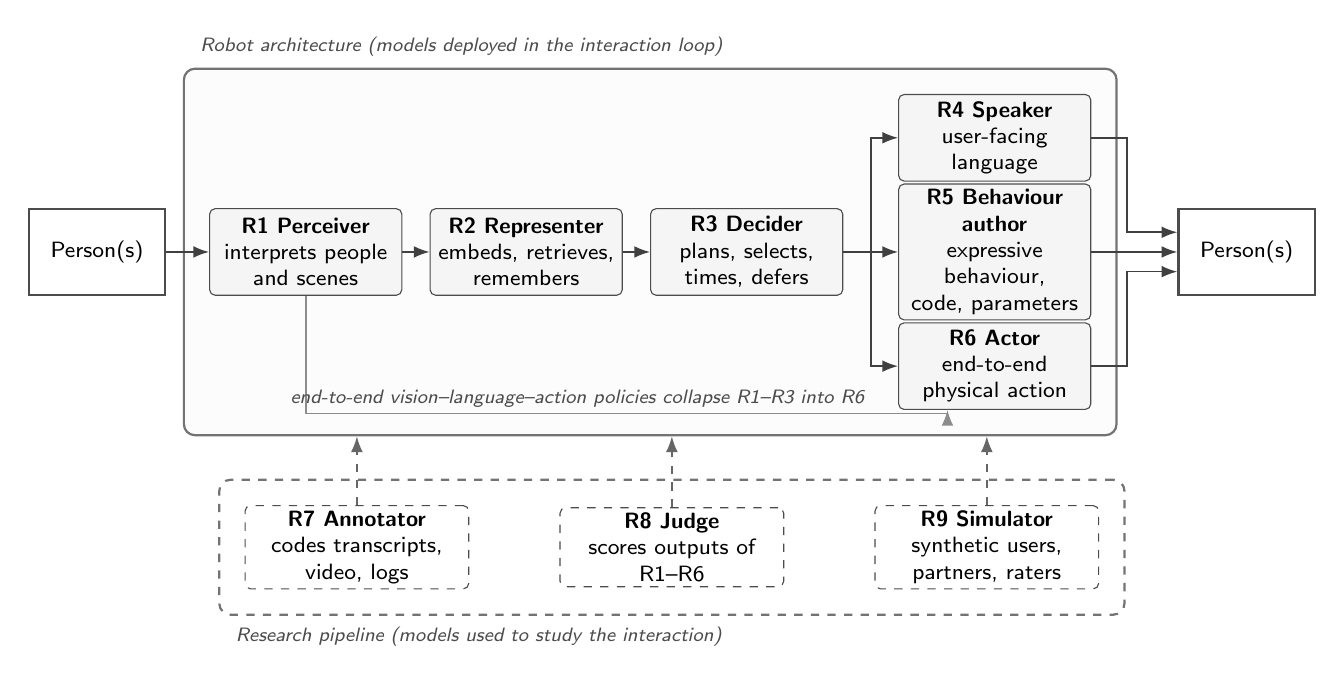
\begin{tikzpicture}[
    font=\sffamily\footnotesize,
    role/.style={draw=black!70, rounded corners=2pt, minimum height=11mm,
                 text width=23mm, align=center, fill=black!4, inner sep=2pt},
    inst/.style={draw=black!70, dashed, rounded corners=2pt, minimum height=9mm,
                 text width=27mm, align=center, fill=white, inner sep=2pt},
    actor/.style={draw=black!70, thick, minimum height=11mm, text width=15mm,
                  align=center, fill=white},
    flow/.style={-{Latex[length=2mm]}, semithick, black!75},
    obs/.style={-{Latex[length=2mm]}, semithick, dashed, black!60},
    band/.style={font=\sffamily\scriptsize\itshape, text=black!70}]

% --- actors --------------------------------------------------------------
\node[actor] (human) at (0,0) {Person(s)};
\node[actor] (human2) at (14.6,0) {Person(s)};

% --- in-robot roles ------------------------------------------------------
\node[role] (perc) at (2.65,0) {\textbf{R1 Perceiver}\\interprets people\\and scenes};
\node[role] (rep)  at (5.45,0) {\textbf{R2 Representer}\\embeds, retrieves,\\remembers};
\node[role] (plan) at (8.25,0) {\textbf{R3 Decider}\\plans, selects,\\times, defers};
\node[role] (lang) at (11.4,1.45) {\textbf{R4 Speaker}\\user-facing\\language};
\node[role] (beh)  at (11.4,0) {\textbf{R5 Behaviour author}\\expressive behaviour,\\code, parameters};
\node[role] (act)  at (11.4,-1.45) {\textbf{R6 Actor}\\end-to-end\\physical action};

\draw[flow] (human) -- (perc);
\draw[flow] (perc) -- (rep);
\draw[flow] (rep) -- (plan);
\draw[flow] (plan.east) -- ++(0.35,0) |- (lang.west);
\draw[flow] (plan.east) -- (beh.west);
\draw[flow] (plan.east) -- ++(0.35,0) |- (act.west);
\draw[flow] (lang.east) -- ++(0.45,0) |- ([yshift=2.5mm]human2.west);
\draw[flow] (beh.east) -- (human2.west);
\draw[flow] (act.east) -- ++(0.45,0) |- ([yshift=-2.5mm]human2.west);

% robot boundary
\begin{scope}[on background layer]
  \node[draw=black!55, thick, rounded corners=4pt, fill=black!1,
        fit=(perc)(rep)(plan)(lang)(beh)(act), inner sep=3.2mm] (robot) {};
\end{scope}
\node[band, anchor=south west] at ([xshift=1mm,yshift=0.2mm]robot.north west)
     {Robot architecture (models deployed in the interaction loop)};

% end-to-end bypass (VLA)
\draw[flow, black!45] (perc.south) |- (act.west |- 0,-2.05) -| ([xshift=-6mm]act.south);
\node[band] at (6.1,-1.86) {end-to-end vision--language--action policies collapse R1--R3 into R6};

% --- research-instrument roles ------------------------------------------
\node[inst] (anno) at (3.3,-3.75) {\textbf{R7 Annotator}\\codes transcripts,\\video, logs};
\node[inst] (judge) at (7.3,-3.75) {\textbf{R8 Judge}\\scores outputs of\\R1--R6};
\node[inst] (sim) at (11.3,-3.75) {\textbf{R9 Simulator}\\synthetic users,\\partners, raters};

\begin{scope}[on background layer]
  \node[draw=black!55, thick, dashed, rounded corners=4pt,
        fit=(anno)(judge)(sim), inner sep=3.2mm] (lab) {};
\end{scope}
\node[band, anchor=north west] at ([xshift=1mm,yshift=-0.2mm]lab.south west)
     {Research pipeline (models used to study the interaction)};

\draw[obs] (anno.north) -- (anno.north |- robot.south);
\draw[obs] (judge.north) -- (judge.north |- robot.south);
\draw[obs] (sim.north) -- (sim.north |- robot.south);
\end{tikzpicture}}
\caption{Nine functional roles that language, vision, and action models play in
HRI research. Solid boxes (R1--R6) are roles inside the robot's interaction
loop; dashed boxes (R7--R9) are roles inside the research pipeline that
observes, scores, or stands in for the interaction. A single model usually
occupies several roles at once, and each role inherits a different evaluation
tradition (Table~\ref{tab:roles}).}
\Description{A block diagram. A person on the left feeds into a chain of three
boxes inside a robot boundary labelled R1 Perceiver, R2 Representer and R3
Decider. The Decider fans out to three output boxes, R4 Speaker, R5 Behaviour
author and R6 Actor, each of which points to a person on the right. A grey
arrow bypasses the chain from the Perceiver to the Actor to indicate
end-to-end vision-language-action policies. Below the robot boundary, a dashed
boundary labelled research pipeline contains three dashed boxes, R7 Annotator,
R8 Judge and R9 Simulator, with dashed arrows pointing up at the robot.}
\label{fig:roles}
\end{figure}


\begin{table}[t]
\caption{Functional roles of generative models in HRI, the evaluation
tradition each inherits, and the component-level evidence that the tradition
treats as the minimum.}
\label{tab:roles}
\small
\begin{tabularx}{\textwidth}{@{}L{2.25cm}L{3.6cm}L{2.9cm}Y@{}}
\toprule
Role & Typical use in HRI & Inherited tradition & Minimum component-level evidence \\
\midrule
\role{1} Perceiver & Infers affect, engagement, intent, or wellbeing from
speech, text, or video; describes scenes & Classification; clinical and
behavioural assessment & Per-class performance against multiply rated human
reference; agreement relative to the human ceiling; subgroup error rates \\
\role{2} Representer & Embeds utterances or images for retrieval, memory,
similarity, clustering, user modelling & Information retrieval; construct
validity & Retrieval accuracy; stability across embedding models and seeds;
null baselines; human check of derived structure \\
\role{3} Decider & Selects plans, skills, or tools; decides when to speak,
help, interrupt, ask, or defer & Planning; judgement and decision-making &
Agreement with expert decisions; constraint violations; calibration of
abstention and help-seeking \\
\role{4} Speaker & Generates language delivered to a person as speech or text
& Human evaluation of generated text and dialogue & Rubric-based ratings by
trained raters with reliability; error taxonomy with severity; audit of
delivered outputs \\
\role{5} Behaviour author & Generates gestures, facial expressions, motion
parameters, or robot programs & Behaviour-perception studies; program
verification & Recognition by naive observers against chance; executability
and safety checks; comparison with expert-authored behaviour \\
\role{6} Actor & Maps observation and instruction directly to motor commands &
Trial-based policy evaluation; safety engineering & Success rates with
intervals over specified conditions; failure taxonomy; safety-envelope
violations; reliably adjudicated outcomes \\
\midrule
\role{7} Annotator & Codes transcripts, video, or logs produced by a study &
Content analysis & Agreement with independent human coders on a held-out
subset, alongside human--human agreement \\
\role{8} Judge & Scores outputs of \role{1}--\role{6} in place of human raters
& Meta-evaluation & Judge--human agreement per construct; bias probes;
independence from the system judged \\
\role{9} Simulator & Stands in for users, partners, or raters & Simulation
validity & Fidelity against human data on the properties relied upon;
restricted to piloting and stress-testing \\
\bottomrule
\end{tabularx}
\end{table}

Three properties of the taxonomy are worth stating. First, roles are
functional, not architectural. A single call to a multimodal model can occupy
several roles at once, as when a model receives a camera frame and a
transcript, decides that the user is distressed (\role{1}), chooses to offer
support instead of continuing the task (\role{3}), and writes the utterance
(\role{4}). The evaluation obligations of all three roles apply, even though
there is one prompt and one output. End-to-end vision-language-action
policies make the same point more sharply: they collapse perception,
representation, and decision into action, which removes the intermediate
outputs that the first three traditions evaluate and leaves only behaviour to
be judged.

Second, the taxonomy makes concrete the contrast with which this article
began. A model in the Speaker role produces open-ended text that a person
hears, so the relevant standard is human evaluation of generated language:
is it relevant, correct, safe, and transparent? A model in the Representer or
Perceiver role produces a vector or a label that a person never sees, so the
relevant standard is that of a measurement instrument or a classifier: is it
accurate against a reliable reference, stable, and unbiased across groups?
Applying the first standard to the second role produces vague reassurance
(``the outputs looked reasonable''); applying the second to the first produces
false precision (an accuracy figure for something that has no single correct
answer).

Third, the research-pipeline roles are included because they are where
generative models have entered HRI most quietly. A study with a fully
scripted robot can still depend on a language model that coded the
transcripts, a vision-language model that scored engagement from video, or
simulated users that were used to tune the protocol. The robot in such a
study is not ``LLM-powered'', and the paper may not appear in any review of
LLM-based HRI, yet its findings are conditional on the model's validity as an
instrument.

\subsection{Four Levels of Evidence}
\label{sec:levels}

Evidence about a model in a role can be gathered at four levels
(Table~\ref{tab:levels}).

\begin{description}[leftmargin=1.2em, style=sameline]
\item[L1 Component.] The model's outputs are evaluated against the standard of
the role's tradition, offline or from logs: are the labels accurate, the
utterances appropriate, the plans executable, the trajectories successful?
\item[L2 System.] The model is evaluated as integrated in the robot and
running in real time: latency, propagation of speech-recognition and
perception errors, consistency between what the model says and what the body
can do, behaviour under network loss, recovery from failure.
\item[L3 Interaction.] People interact with the robot and outcomes are
measured in them: perceptions, behaviour, task performance, learning,
wellbeing. This is the level of the HRI user study.
\item[L4 Deployment.] The robot is used over time outside the laboratory:
drift in model behaviour, novelty effects, accumulation of memory and
personalisation, rare harms, and the organisational context of use.
\end{description}

\begin{table}[t]
\caption{Questions answered at each level of evidence, with typical measures.
The levels are complementary: evidence at one level does not substitute for
evidence at another.}
\label{tab:levels}
\small
\begin{tabularx}{\textwidth}{@{}L{1.9cm}L{4.3cm}Y@{}}
\toprule
Level & Question & Typical measures \\
\midrule
L1 Component & Are the model's outputs adequate for the role? & Agreement
with human reference; rubric ratings; accuracy, F1, calibration; success rate
over trials; error and hallucination rates; run-to-run and prompt-to-prompt
consistency \\
L2 System & Does the integrated robot behave as specified in real time? &
End-to-end response latency distribution; word error rate and its downstream
effect; capability-consistency violations; fallback and timeout rates;
intervention rate of a supervising human \\
L3 Interaction & What happens to the people who interact with it? &
Validated self-report scales; behavioural measures; task outcomes;
manipulation checks; qualitative accounts; adverse events \\
L4 Deployment & Does it keep working, and for whom, over time? & Longitudinal
outcome trajectories; usage and attrition; drift under model updates; incident
reports; subgroup differences in benefit and harm \\
\bottomrule
\end{tabularx}
\end{table}

The central principle is that \emph{evidence does not transfer between levels
without an argument}. Two inferential errors follow from ignoring it, and both
are common.

The \emph{upward leap} takes component-level evidence, often not even the
authors' own, as support for interaction-level claims. A model that leads a
public benchmark, or that the authors found to give sensible answers when
prompted at a desk, is assumed to be adequate when embodied in a robot,
addressed in noisy speech by an older adult, and constrained to answer within
a conversational pause. Benchmarks rarely sample that context, and the
system-level properties that decide whether an interaction succeeds, such as
latency and error propagation, are not properties of the model at all.

The \emph{downward leap} takes interaction-level evidence as support for
component-level adequacy. Participants rated the robot as empathic,
trustworthy, and useful, so its utterances are taken to have been accurate
and safe. This inference fails for a specific reason: participants are poorly
placed to detect the errors that matter most. A fluent, confident, incorrect
answer is by construction one that the listener does not recognise as
incorrect. Favourable questionnaire scores are compatible with a robot that
fabricated facts, overstated its capabilities, or gave advice a professional
would not have given. Only an audit of the outputs that participants actually
received can establish what they received.

\subsection{Five Kinds of Claim}
\label{sec:claims}

Evaluation serves a claim, and the same data can be adequate for one claim
and inadequate for another. We distinguish five.

\begin{description}[leftmargin=1.2em, style=sameline]
\item[Capability.] The model can perform the role to a stated standard under
stated conditions (``the model classified engagement with $F_1=.78$ against
two trained coders'').
\item[Comparison.] One configuration performs differently from another on a
stated outcome (``participants disclosed more to the robot with the adaptive
prompt than to the robot with the static prompt'').
\item[Substitution.] The model can replace a human, or a more expensive
procedure, for a stated purpose (``the model can replace the second coder'';
``the autonomous robot can replace the wizard'').
\item[Safety.] The frequency and severity of harmful outputs or actions are
below a stated bound under stated conditions.
\item[Generalisation.] A finding obtained with one model, prompt, population,
or setting holds for others.
\end{description}

Substitution and safety claims carry the heaviest burden and are the most
often under-supported. A substitution claim is a claim of equivalence or
non-inferiority, and a non-significant difference between model and human in a
small sample is not evidence of either (Section~\ref{sec:equivalence}). A
safety claim concerns the tail of a distribution, and a mean rating says
little about tails. Generalisation claims about ``LLMs'' or ``VLAs'' as a
class, made on the basis of one model at one point in time, are best avoided
or explicitly hedged; what a study shows is that one configuration behaved in
one way.

\subsection{Three Tiers of Proportionate Evidence}
\label{sec:tiers}

Not every use of a model deserves the same scrutiny, and a standard that
demanded maximal evidence everywhere would be ignored everywhere. We propose
that the evidence expected of a study scale with three questions: who is
\emph{exposed} to the model's output and how directly, what is the worst
plausible \emph{consequence} of an inadequate output and can it be reversed,
and how much \emph{oversight} stands between the output and the person.
Table~\ref{tab:tiers} gives three tiers. A study is assigned the highest tier
that any of its roles reaches.

\begin{table}[t]
\caption{Three tiers that scale the expected evidence to exposure,
consequence, and oversight.}
\label{tab:tiers}
\small
\begin{tabularx}{\textwidth}{@{}L{1.8cm}L{4.6cm}Y@{}}
\toprule
Tier & Defining conditions & Expected in addition to the tier below \\
\midrule
I Exploratory & Outputs are reviewed by a researcher before use, or reach
only informed adult participants in low-stakes tasks under supervision;
errors are harmless and reversible; claims are of capability or feasibility &
Role, level, and claim declared; model and configuration fully reported;
outputs logged and a sample inspected and described; limits on the claim
stated \\
II Standard & Outputs reach participants unreviewed in a controlled study, or
model-produced labels and scores feed the study's inferential statistics;
claims are comparative & Component-level validation against a human reference
with reliability statistics; repeated-run consistency; audit of delivered
outputs; validated automated evaluators; uncertainty intervals \\
III High-stakes & Outputs reach children, patients, older adults, or people in
distress; or drive physical action near people; or operate unsupervised over
time; or support substitution or safety claims & Domain-expert raters;
pre-registered evaluation plan; subgroup and failure-tail analysis; adversarial
and stress testing; system-level safety measures with logged human
intervention; monitoring plan for deployment \\
\bottomrule
\end{tabularx}
\end{table}

The tiers are deliberately coarse. Their purpose is to give authors and
reviewers a shared starting point for the question ``is this enough?'', and to
make explicit that the answer depends on the role and the stakes and not on
which model was used. A late-breaking report that explores whether a
vision-language model can describe a robot's workspace need not meet the bar
set for an autonomous robot that conducts wellbeing conversations with
adolescents; but the second study should not be reviewed as if it were the
first.

\section{Practices for Every Study}
\label{sec:crosscutting}

Ten practices apply whatever role the model plays. They are stated as
imperatives for brevity; the tier scheme of Section~\ref{sec:tiers} governs
how far each should be taken.

\subsection{Say What the Model Is Doing and What Is Being Claimed}

\begin{practice}{bp:declare}{Declare roles, levels, and claims}
State every role each model plays, in the robot and in the analysis; state at
which levels evidence was gathered; and state which claims the evidence is
offered for.
\end{practice}

The declaration costs a paragraph and removes the most common obstacle to
assessing an LLM-based HRI paper, which is not knowing what the model did.
Phrases such as ``the robot was powered by GPT-4'' conceal whether the model
generated every utterance verbatim, selected among scripted utterances,
paraphrased a script, produced labels that a rule-based dialogue manager
consumed, or drafted text that an experimenter approved. These are different
roles with different risks. The declaration should include roles in the
research pipeline, and it should say which outputs reached participants
without human review.

\subsection{Report the Configuration as the Stimulus}

\begin{practice}{bp:config}{Report the full configuration}
Report the model snapshot, provider, access dates, sampling parameters,
complete prompts, injected context, tools, memory, guardrails, and the speech
and perception components around the model, in enough detail for another
laboratory to reconstruct the stimulus.
\end{practice}

In an experiment the robot's behaviour is the stimulus, and with a generative
model the stimulus is produced by the conjunction of model weights, prompt,
context, and sampling parameters. Omitting any of them is equivalent to not
describing the stimulus. Three facts make this more than a formality. Hosted
models change: the measured behaviour of the same named commercial model on
the same tasks shifted substantially within months \cite{chen2024how}, so a
product name without a dated snapshot identifies a moving target. Hosted
models are withdrawn, which makes exact replication impossible and is a
principal argument for justifying any reliance on proprietary models in
research \cite{palmer2024using,ollion2024dangers,rogers2023closed}. And
outputs are sensitive to prompt details that authors regard as incidental:
changes of formatting alone, with meaning held constant, moved one model's
accuracy by as much as 76 points \cite{sclar2024quantifying}.

For robots, the configuration extends beyond the model. The system prompt
usually carries the robot's persona, its stated capabilities, and its
behavioural boundaries, and is therefore part of the design under study.
Expert consultation at RO-MAN 2025 produced a template with eight functional
components for specifying, bounding, and adapting robot behaviour through
prompts, proposed explicitly as a reporting aid as well as a design aid
\cite{ashok2026why}; we recommend its use. The pipeline around the model
(speech recogniser, voice-activity detection, text-to-speech, the mapping from
model output to gesture, any content filter and what the robot does when the
filter fires) shapes what the participant experiences as much as the model
does and should be reported with it. For action models, the checkpoint,
fine-tuning data, embodiment, control frequency, and the safety layer between
policy and actuators are the corresponding items. Experiment platforms that
store prompts and configurations alongside interaction logs make such
reporting a by-product of running the study \cite{laban2024lexi}.

\subsection{Measure Consistency Before Measuring Anything Else}

\begin{practice}{bp:consistency}{Measure run-to-run and prompt-to-prompt consistency}
Run the model more than once on the same inputs, and with reasonable variants
of the prompt, and report how much its outputs or scores vary.
\end{practice}

Psychometrics holds that reliability bounds validity: an instrument that does
not agree with itself cannot agree with anything else. A human coder is asked
to demonstrate intra-rater reliability by coding the same material twice. The
same should be asked of a model, and it frequently is not. Generative models
are stochastic by default, and configuring a hosted model to be
deterministic does not make it so: across ten runs of five such models,
accuracy varied by up to 15\% \cite{atil2025nondeterminism}.
Repeated classification of identical texts by the same model with the same
prompt can fall below conventional reliability thresholds
\cite{reiss2023testing}, model judges asked to rate the same output
repeatedly have shown low intra-rater reliability, in the worst case close to
arbitrary \cite{haldar2025rating,schroeder2024can}, and conclusions drawn
from a single prompt often do not survive paraphrase of the instruction: in
an evaluation of twenty models on thirty-nine tasks, paraphrasing the
instruction changed both absolute and relative performance
\cite{mizrahi2024state}.

In practice this means, for a model that labels or scores (\role{1},
\role{7}, \role{8}), running each item several times and reporting the
agreement among runs with the coefficient that will later be used for
agreement with people, so that the two are comparable. As a working default
we suggest five runs, increased when agreement among them is below the level
required of human coders. For a model that generates (\role{4}, \role{5}),
consistency concerns properties and not surface form: across repeated
generations from the same context, how often does the response satisfy each
criterion of the rubric, and how often does it contain a serious error? For a
model that decides or acts (\role{3}, \role{6}), it is the repeatability of
outcomes from nominally identical initial conditions. Agent benchmarks have
begun to report this as a quantity in its own right, the probability that a
task is completed on all of $k$ independent attempts, and find it far below
single-attempt success \cite{yao2025taubench}; gains in capability across
model generations have brought only small gains in reliability so defined
\cite{rabanser2026towards}. For a robot that someone will rely on daily,
succeeding every time is the property of interest. Where the study's conclusion depends on a
prompt, at least a small set of meaning-preserving variants should be tested
and the spread reported. Section~\ref{sec:gtheory} describes a design that
estimates these sources of variance jointly.

\subsection{Build a Human Reference and Show That It Is Reliable}

\begin{practice}{bp:human}{Establish a human reference with documented reliability}
Have at least two suitably qualified people independently rate or code the
material against a written rubric, report their agreement with an appropriate
coefficient and its confidence interval, and treat that agreement as the
ceiling against which the model is read.
\end{practice}

Human judgement is the reference for almost everything HRI wishes to know
about a model's outputs, and it is only as good as its reliability. Reviews
of human evaluation in natural language generation document how often this
is neglected: studies omit the number of raters, their expertise, the
question they were asked, and any measure of agreement
\cite{vanderlee2021human}. An annotation of 165 NLG papers found more than
200 different terms for the quality aspects being evaluated
\cite{howcroft2020twenty}, which later work has tried to consolidate into a
standard set of named and defined criteria \cite{belz2025standard}; a review
of 135 papers found that most reported agreement fell short of conventional
thresholds \cite{amidei2019agreement}; and when published human evaluations
were selected for reproduction, only 13\% provided enough information to
attempt it, and flaws were found in nearly all that were attempted
\cite{belz2023missing,thomson2024common}. Neighbouring fields are little better: in a sample
of qualitative papers from CSCW and HCI venues, inter-rater reliability was
reported in about one in nine \cite{mcdonald2019reliability}. HRI, which has
a long practice of behavioural coding, is well placed to do better, but the
practice needs adapting in four respects.

\paragraph{Choose the coefficient to fit the data.} Table~\ref{tab:irr}
summarises the choice. Percentage agreement should not be reported alone
because it does not correct for chance \cite{cohen1960coefficient,
hallgren2012computing}. Krippendorff's $\alpha$ handles any number of raters,
missing ratings, and nominal to ratio data, and is the most generally
applicable single choice \cite{hayes2007answering,krippendorff2019content}.
For continuous ratings the intraclass correlation is appropriate, provided
the model (one-way or two-way, random or mixed), the type (consistency or
absolute agreement), and the unit (single or average rating) are stated,
since these change the value and its meaning
\cite{shrout1979intraclass,koo2016guideline}.

\begin{table}[t]
\caption{Choosing an agreement statistic for a human reference, or for
comparing a model with one. In every case report the number of raters and
items, the prevalence of each category, and a confidence interval.}
\label{tab:irr}
\small
\begin{tabularx}{\textwidth}{@{}L{3.6cm}L{4.4cm}Y@{}}
\toprule
Data & Statistic & Notes \\
\midrule
Nominal labels, two raters & Cohen's $\kappa$
\cite{cohen1960coefficient} & Sensitive to prevalence and to differences in
raters' marginals; add per-category agreement \\
Nominal labels, more than two raters or missing ratings & Krippendorff's
$\alpha$ \cite{hayes2007answering}; Fleiss' $\kappa$
\cite{fleiss1971measuring} & $\alpha$ accommodates incomplete designs \\
Ordinal ratings (e.g.\ rubric scores) & Weighted $\kappa$
\cite{cohen1968weighted}; ordinal $\alpha$ & State the weighting scheme \\
Continuous or scale ratings & Intraclass correlation
\cite{shrout1979intraclass,koo2016guideline} & State model, type, and unit;
use absolute agreement when the values will be used as scores \\
Rare categories (e.g.\ safety violations) & $\kappa$ or $\alpha$ with
prevalence, positive and negative agreement; Gwet's AC1
\cite{gwet2008computing} & High raw agreement can coexist with low $\kappa$
\cite{feinstein1990high,byrt1993bias} \\
Two measurement methods on a continuous quantity & Bland--Altman limits of
agreement \cite{bland1986statistical}; concordance correlation
\cite{lin1989concordance} & Correlation alone ignores systematic offset \\
Interpretive qualitative analysis & Agreement statistics may be
inappropriate \cite{mcdonald2019reliability,braun2019reflecting} & Report the
analytic approach and how rigour was pursued instead \\
\bottomrule
\end{tabularx}
\end{table}

\paragraph{Interpret the value in context.} The verbal bands commonly
attached to $\kappa$ (``moderate'', ``substantial'') were offered by their
authors as arbitrary conveniences \cite{landis1977measurement}, and
Krippendorff's often-cited guidance to rely on variables with
$\alpha\geq.800$ and to draw only tentative conclusions from those between
.667 and .800 was offered for content analysis in general
\cite{krippendorff2019content}. Neither is a pass mark, and for subjective
judgements a fixed threshold is hard to defend at all; an alternative is to
benchmark agreement against a replication of the human rating itself
\cite{wong2021crossreplication}. What matters is the
consequence of the residual disagreement for the use to which the ratings are
put, and for that the confidence interval is as important as the point
estimate. Table~\ref{tab:kappa} in the Appendix shows that with a hundred
double-coded items, a common size for a validation subset in HRI, an observed
$\kappa$ of .60 is compatible with true values from roughly .44 to .74 when
categories are balanced, and with a much wider range when one category is
rare.

\paragraph{Watch prevalence.} The categories of greatest interest in HRI are
often rare: the unsafe utterance, the distressed child, the hazardous motion.
When a category is rare, raters who agree on nearly every item can have a low
$\kappa$, and, conversely, high raw agreement can conceal an inability to
agree on the rare cases at all \cite{feinstein1990high,byrt1993bias}. A
robot-led assessment of children's wellbeing with a vision-language model
illustrates the point from the model's side: the model agreed with a
psychologist on about 82\% of the items where no concern was coded, but on
only about 13\% of the items where a concern was coded, for a Cohen's
$\kappa$ of .22 \cite{abbasi2025robotled}. Overall agreement would have
suggested a serviceable instrument. Per-category agreement showed one that
missed most of what it was deployed to find.

\paragraph{Decide what disagreement means.} For some constructs disagreement
between raters is noise to be reduced by training and a sharper codebook. For
others, including many that HRI cares about (was that response empathic? was
that interruption rude? was that gesture appropriate?), disagreement reflects
real differences between people and cultures, and collapsing it into a
majority label discards information and installs one group's view as ground
truth \cite{aroyo2015truth,plank2022problem,uma2021learning}. For such
constructs we recommend reporting the distribution of ratings, recruiting
raters from the populations the robot is meant to serve, and evaluating
models against the distribution (Section~\ref{sec:perspectivist}).

Two further points concern who the raters are. Expertise should match the
construct: the clinical appropriateness of a wellbeing robot's response is a
matter for clinically trained raters, and lay raters have been shown to be
unreliable judges even of whether text was written by a person
\cite{clark2021all} and of the quality of open-ended generated text
\cite{karpinska2021perils}. And raters should be blind to the source of what
they rate (model or human, and which condition), since knowledge of the
source shapes judgement.

\subsection{Validate Automated Evaluators Before Relying on Them}

\begin{practice}{bp:validate}{Validate every automated evaluator against the human reference}
Before a metric, a model judge, or a model annotator is used to support a
claim, demonstrate on held-out, human-rated material from the study's own
domain that it agrees with people about as well as people agree with each
other.
\end{practice}

Automatic evaluation is attractive in HRI for the same reason as elsewhere:
human rating is slow and expensive. Its history in dialogue research is a
caution. Word-overlap metrics imported from machine translation were found to
correlate weakly or not at all with human judgements of dialogue responses
\cite{liu2016how}, yet were reported for years. Model-based judges are far
more capable, and on some tasks reach agreement with human preferences
comparable to agreement between humans \cite{zheng2023judging,chiang2023can}.
But the evidence for them is uneven across tasks: a study spanning twenty NLP
datasets found large variation in how well model judgements tracked human
ones and concluded that judges need to be validated for each task before use
\cite{bavaresco2025llms}. Even where humans agree strongly with one
another, only the best of thirteen judge models aligned reasonably with them
and none reached the level of agreement among humans, and judges with high
percentage agreement still assigned very different scores
\cite{thakur2025judging}. Without a correct reference answer, judges agreed
with experts mainly on the questions they could answer themselves
\cite{krumdick2026no}. Judges also have systematic biases, including
sensitivity to the order in which candidates are presented
\cite{wang2024large}, a preference for text produced by the judging model
itself \cite{panickssery2024llm}, and a range of other cognitive-bias
analogues \cite{koo2024benchmarking}.

Validation on HRI material has only begun, and what there is counsels
caution. When language models were asked to reproduce participants'
responses in three published HRI user studies, the strongest model
correlated highly with people in two of them and no model did in the third;
vision-capable models failed on the video stimuli; and models rated robot
behaviour more favourably than people had \cite{wachowiak2024are}. When
models completed standard HRI questionnaires for a set of recorded
interactions, they agreed moderately to strongly with human observers on
engagement and were highly consistent from run to run, yet their ratings of
comfort and strangeness were \emph{inversely} related to those of people
\cite{lockwood2026when}. The second result deserves emphasis because it
separates two things that are easily conflated: the models were reliable,
and on that dimension they were wrong. The constructs that HRI most often
asks a judge to score (social appropriateness in a physical context,
fidelity to a therapeutic technique, consistency between an utterance and
what the robot's body is doing) and the inputs it most often supplies
(transcripts of recognised speech with errors, video of a robot and a
person) remain largely unvalidated. A judge's validity is specific to the construct, the rubric, the
prompt, and the kind of material. It has to be established locally, on the
study's own data, with the study's own rubric, and the role-specific
practices for Annotators and Judges (\bpr{bp:coder}, \bpr{bp:judge}) say how.

\subsection{Quantify Uncertainty and Plan for Precision}

\begin{practice}{bp:uncertainty}{Report uncertainty and size evaluations deliberately}
Attach an interval to every component-level estimate, choose the number of
items, trials, raters, and runs in advance on the basis of the precision
required, and analyse nested data as nested.
\end{practice}

Component-level results in HRI papers are frequently single numbers from
small samples. The statistical literatures of both NLP and robot learning have
argued at length that this is inadequate: significance testing and power
analysis are underused in NLP \cite{dror2018hitchhikers,card2020with}, model
evaluations are experiments whose results need standard errors
\cite{miller2024adding}, error bars based on the central limit theorem
understate uncertainty for evaluation sets of fewer than a few hundred items
\cite{bowyer2025position}, and reports of robot policy performance from a
handful of trials do not support the comparisons drawn from them
\cite{kressgazit2024robot,agarwal2021deep}. Table~\ref{tab:cp} in the Appendix
makes the last point concrete.

Two features of HRI data need particular care. The data are nested: turns
within sessions within participants, trials within objects within scenes.
Treating five hundred robot utterances from twenty participants as five
hundred independent observations overstates precision; mixed-effects models
or cluster bootstraps are the appropriate tools, as they are for the
participant-level outcomes of the same studies. And evaluation sets are
typically built after the fact from whatever the study produced. Deciding in
advance how many items will be double-coded, how they will be sampled
(stratified by session, participant, and condition, with over-sampling of rare
categories), and what interval width is acceptable turns validation from a
ritual into a measurement.

\subsection{Disaggregate}

\begin{practice}{bp:subgroup}{Report performance for the groups of people the robot serves}
Break component-level performance down by participant characteristics
relevant to the application, and test whether error rates differ.
\end{practice}

Aggregate performance can hide failure concentrated in a subgroup, and
embodiment gives such failure direct consequences. Robots driven by
foundation models have been shown to act on social stereotypes
\cite{hundt2022robots}, and LLMs prompted in HRI scenarios produce
discriminatory outputs across protected characteristics and accept harmful
instructions \cite{hundt2025llm}. In the child wellbeing assessment discussed
above, the vision-language model's false-positive rate was significantly
higher for girls than for boys, so that it failed the equalised-odds criterion
even when gender was not mentioned in the prompt \cite{abbasi2025robotled}.
Speech recognition, which sits upstream of most spoken HRI, has well-documented
disparities by speaker group \cite{koenecke2020racial}, and an error there
becomes an error in everything the language model does next. HRI samples are
small and not diverse \cite{seaborn2023not}, which limits what
disaggregation can show; but reporting the breakdown, with intervals, allows
later synthesis, and its absence should be stated as a limitation and not
passed over.

\subsection{Characterise Failures, Not Only Averages}

\begin{practice}{bp:failures}{Report an error taxonomy, severity, and the worst cases}
Classify the model's errors by type and by severity for the person, report the
frequency of each, and describe the most serious individually.
\end{practice}

A mean rubric score of 4.3 out of 5 is uninformative about whether the robot
once told a participant something dangerous. HRI has taxonomies of robot
failure and of social error that can be extended to generative components
\cite{honig2018understanding,tian2021taxonomy}, and the NLP literature
supplies taxonomies of hallucination \cite{ji2023survey}. Failure modes that
studies of LLM-driven robots have documented, and that a taxonomy for HRI
should therefore include, are fabricated facts and memories, claims to
capabilities or experiences the robot does not have, loss of persona or of
conversational context, responses that are too long or too late for spoken
interaction, misrecognised speech treated as intended, and inappropriate
advice \cite{irfan2025between,ashok2026why}. For action models the
corresponding list includes hesitation, motion that is successful but
illegible or alarming, and task success achieved in a way that would be
unacceptable around a person \cite{guan2024task}. Severity should be rated
separately from frequency and with reference to the population: the same
error has different weight for a student volunteer and for a person with
dementia.

\subsection{Connect the Levels}

\begin{practice}{bp:levels}{Audit what participants actually received, and measure the system around the model}
Log every model output delivered in the study and evaluate those outputs, or a
defined sample of them, at component level; report system-level properties
that mediate between model and person; and verify manipulations in the
delivered outputs.
\end{practice}

This practice answers the two inferential leaps of
Section~\ref{sec:levels}. Against the downward leap, it requires that
outputs produced \emph{in situ} be audited, since outputs produced at the
desk before the study are not the outputs participants heard. A generative
model makes every participant's interaction different; the audit is the only
means of knowing what the ``treatment'' was. It also supplies the
manipulation check that experimental method requires
\cite{hoffman2021primer}: if two conditions differ in a prompt intended to
make the robot more empathic, the audit should show that raters blind to
condition find its utterances more empathic.

Against the upward leap, it requires measurement of what lies between model
and person. Response latency is the clearest case. Gaps between turns in
human conversation are typically a few hundred milliseconds across languages
\cite{stivers2009universals}, and timing is central to how spoken interaction
with machines is experienced \cite{skantze2021turn}; a pipeline of speech
recognition, a hosted model, and speech synthesis commonly takes several
times longer, and the delay, the filler that masks it, and the interruptions
it causes are part of the stimulus. The distribution of latency, and not only
its mean, should be reported. So should the word error rate of the speech
recogniser in the study's acoustic conditions and with the study's
population, since recognition errors are a leading cause of breakdown in
LLM-driven conversation with older adults \cite{irfan2025between}.

Where a human supervises the robot, their interventions are data. Riek's
guidelines for Wizard-of-Oz studies asked authors to report what the wizard
could do, what they did, and how they were trained \cite{riek2012wizard}.
Supervised autonomous systems need the equivalent: under what conditions the
supervisor could veto, edit, or replace an output, how often they did, and
why. The intervention rate is among the most informative system-level
measures of a generative component's readiness, and it is almost free to
collect.

\subsection{Preserve, Share, and Pre-Specify}

\begin{practice}{bp:open}{Archive the materials and fix the evaluation plan in advance}
Preserve prompts, configurations, interaction logs, rater data, and judge
outputs; share what consent and privacy allow; and specify prompts, rubrics,
judges, validation subsets, and thresholds before the evaluation is run.
\end{practice}

Generative models multiply the analytic choices available to a researcher.
The prompt can be reworded, the model swapped, the temperature changed, the
rubric adjusted, the judge replaced, each change producing a somewhat
different result. The lesson of the replication crisis in psychology is that
undisclosed flexibility of this kind reliably produces false positives
\cite{simmons2011falsepositive}. The same has now been shown for model
configurations. In a replication of 37 annotation tasks from 21 social
science studies, using 18 models and some 13 million labels, the choice
among defensible configurations led to incorrect conclusions for roughly a
third of hypotheses even with state-of-the-art models, and a few
paraphrases of the prompt were enough to make almost any result significant
\cite{baumann2025large}. Re-running one published use of simulated
respondents under 66 defensible configurations moved its correlation with
human data from .23 to .84 \cite{cummins2026threat}. Reporting results
across the set of reasonable prompts, models, and decoding settings, as a
multiverse or specification curve
\cite{steegen2016increasing,simonsohn2020specification}, is the transparent
alternative to reporting the configuration that happened to work.
Pre-registration, the remedy psychology adopted \cite{nosek2018preregistration},
transfers directly: the prompt, the model, the rubric, the validation sample,
and the agreement threshold can be fixed and time-stamped before the model is
run on the study data. Prompt development is legitimate, but it should be
done on separate material, and the paper should say so.

Preservation matters more than usual because the model itself cannot be
archived when it is hosted. The interaction logs then become the only
permanent record of what the system did, and a set of archived contexts is
what makes later comparison with a successor model possible
(Section~\ref{sec:replay}). HRI's reproducibility agenda already calls for
sharing code, materials, and data \cite{gunes2022reproducibility}; for
studies with generative models the minimum addition is the complete prompt
set and, where consent permits, de-identified logs. Sending participants'
speech, images, or disclosures to a third-party model provider is a
data-protection matter that belongs in ethics review and in the consent form,
and is a reason, alongside reproducibility, to consider locally run
open-weight models where they are adequate to the role, as was done for the
assessment of children's narratives cited above \cite{abbasi2025robotled}.

\section{Practices for Each Role}
\label{sec:rolepractices}

The fourteen practices in this section are specific to roles. Each adapts the
tradition named in Table~\ref{tab:roles} to the conditions of HRI.

\subsection{R1 Perceiver}

\begin{practice}{bp:perceiver}{Evaluate a perceiving model as a measurement instrument}
Report per-class performance against a reference produced by more than one
qualified rater, express model--human agreement relative to human--human
agreement, and, where the output will inform decisions about a person, meet
the standard expected of an assessment tool.
\end{practice}

Language and vision-language models are used to infer what a robot cannot
sense directly: emotion from a face or a transcript, engagement from video,
intent from an ambiguous request, wellbeing from a child's narrative. This is
classification or scoring, and the intuition that evaluating it looks like
evaluating a classification model is right, with three qualifications that
the affective-computing and psychometric literatures supply.

First, the reference labels are themselves judgements. For affect,
engagement, and rapport there is no instrument-independent truth, only what
trained observers or the person themselves report, and these disagree. The
model cannot be expected to agree with the reference more than the reference
agrees with itself, so human--human agreement must be measured and reported
as the ceiling (\bpr{bp:human}). A reference produced by a single rater, a
frequent economy, makes the ceiling unknown and the model's score
uninterpretable; the authors of the child wellbeing study name their single
psychologist rater as a principal limitation for this reason
\cite{abbasi2025robotled}.

Second, class imbalance is the norm, so accuracy is uninformative and
per-class precision, recall, and agreement are required (\bpr{bp:human},
\bpr{bp:subgroup}).

Third, what the model is given matters as much as which model it is. A model
may receive raw video, a transcript, or features extracted by an upstream
component, such as valence and arousal values computed from facial
expressions and passed to a language model as numbers \cite{mehra2025how}.
Each arrangement has a different error profile, and the evaluation should be
of the arrangement used on the robot, with the robot's sensors, viewpoint,
and lighting, and not of the model on a curated benchmark. The gap can be
large: multimodal models rating emotional arousal from video approached
human-level reliability on laboratory recordings but correlated at best
moderately with human ratings of real-world footage, and showed
gender-differential bias \cite{licht2025computational}.

When a Perceiver's output is used to draw conclusions about an individual
(screening, assessment, adaptation of an intervention), the relevant standard
is that of psychological testing: evidence of reliability, of validity
against an external criterion, and of fairness across groups, for the
intended use and population \cite{aera2014standards}. A model that performs
``reasonably'' on average does not meet it.

\subsection{R2 Representer}

\begin{practice}{bp:embed}{Show that structure derived from embeddings is not an artefact of the embedding}
When embeddings are used to cluster, compare, or measure similarity, repeat
the analysis with more than one embedding model, calibrate similarity against
an empirical null, test the stability of clusters, and have people check the
resulting structure.
\end{practice}

Embeddings have become a standard analytic instrument in HRI as elsewhere:
utterances are embedded, clustered into themes, and the themes labelled by a
language model; or the similarity of two sets of texts is taken as a measure
of how alike two conditions, partners, or populations are. The approach
scales to corpora that could not be coded by hand, and it has produced
findings about what people disclose to robots that would otherwise be
unavailable \cite{chiang2025selfdisclosure,laban2025what}. Its validity rests
on four checks.

\emph{Triangulation.} Cosine similarity is defined relative to an embedding
space. Contextual embedding spaces are anisotropic, so that even unrelated
texts have high cosine similarity in some models
\cite{ethayarajh2019how}, whereas models trained with a sentence-similarity
objective spread texts more widely \cite{reimers2019sentence}. The same pairs
of disclosures were found to have mean similarity below .50 in one family and
above .80 in two others \cite{chiang2025selfdisclosure}. Conclusions should
therefore be reported for at least two embedding families, and those that
hold in only one should be flagged.

\emph{Null calibration.} For the same reason, fixed thresholds are not
portable. The reference point for an observed similarity is the distribution
of similarity between randomly paired items in the same space, or under
permutation of the grouping variable, and the result is best expressed as a
standardised difference from that null.

\emph{Stability.} A clustering is one of many that an algorithm could have
returned. The number of clusters, the random initialisation, and the sample
all move the partition. Reporting how well the clusters are recovered across
seeds and bootstrap resamples, for example by the mean adjusted Rand index or
cluster-wise Jaccard similarity \cite{hennig2007cluster}, distinguishes
structure in the data from structure in the run.

\emph{Human check.} Automatically generated cluster labels are fluent whether
or not the cluster is coherent. Topic-model research met this problem and
devised intrusion tasks, in which people try to spot the item that does not
belong \cite{chang2009reading}. The same test applies to embedding clusters,
alongside a conventional check in which two coders assign a sample of items
to the labelled themes. An automated check that each generated description
lies closest to its own centroid, as used in the studies above, is a useful
necessary condition and costs nothing; it is not a substitute.

\begin{practice}{bp:memory}{Evaluate retrieval and memory as retrieval}
When embeddings select what the robot remembers or retrieves, report
retrieval quality and the rate of retrieving material that should not have
been retrieved, including material about a different person.
\end{practice}

Long-term interaction increasingly relies on retrieval: past conversations or
user facts are embedded, and the most similar are inserted into the prompt.
The retrieval step is an information-retrieval system and can be evaluated as
one, with precision and recall against human judgements of relevance, and
with the faithfulness of the generated response to what was retrieved
\cite{es2024ragas}. HRI adds a failure with social and legal weight:
retrieving one person's disclosure into a conversation with another, in a
household or care home where a robot serves several people. The rate of such
cross-person retrieval should be measured directly.

\subsection{R3 Decider}

\begin{practice}{bp:decider}{Evaluate decisions against expert decisions, and evaluate whether the model knows when not to decide}
Compare the model's choices with those of qualified people in the same
situations using agreement statistics, report violations of stated
constraints, and measure whether the model's abstentions and requests for
help are calibrated to its uncertainty.
\end{practice}

Models decide which skill to execute, which tool to call, and what to do
next in a task plan \cite{ahn2022do,liang2023code}; in social robots they
also decide when to take a turn \cite{skantze2025applying}, and whether a
situation calls for help, silence, or intervention
\cite{tanneberg2024help}. Such decisions are sometimes verifiable (a plan is
executable or not) and sometimes normative (it was or was not appropriate to
interrupt). For the normative kind, the evaluation is a comparison with
people's decisions in the same situations, subject to everything said about
human references above. GRACE shows what such an evaluation looks like when
the reference is taken seriously \cite{dogan2025grace}. It predicts how
socially appropriate each of several household actions (vacuuming, carrying
warm food, starting a conversation) would be in a given scene, and it
evaluates five language models, open-weight and proprietary, against
appropriateness scores given by thousands of human annotators, using error
and two correlation measures, one of which, the concordance correlation
coefficient, penalises systematic offset (Table~\ref{tab:irr}). Two features
make it an exemplar for this role. It does not treat the human scores as a
single truth: scenes are first separated into those on which annotators
agree and those on which they do not, and model performance is reported for
each, which showed that the models tracked human judgement more closely
where people agreed with one another and least closely where they did not.
And it uses the human explanations that accompany the scores to correct the
language model's predictions in the uncertain scenes, which improved
agreement with human scores over the language model alone (for the
strongest model, concordance rose from .23 to .48). The lesson for
evaluation is general: where a Decider's task is normative, performance
should be reported conditional on human agreement, because a model cannot be
right about a scene on which people are divided, only more or less
representative of them (Section~\ref{sec:perspectivist}).

Two cautions apply. A model that predicts human preferences well on
vignettes has been proposed as a zero-shot human model for planning
\cite{zhang2023large}, but apparent social reasoning can be brittle:
performance on theory-of-mind style judgements in HRI scenarios degraded
under perturbations that should not have mattered \cite{verma2024theory}.
Decisions should therefore be tested under perturbation of irrelevant
context as well as on canonical cases. And a Decider should be evaluated on
its uncertainty, because the safe response to ambiguity in HRI is usually to
ask. Conformal prediction has been used to make an LLM planner request human
help at a rate tied to a specified level of task success
\cite{ren2023robots}. Whether or not such machinery is used, the rate at
which the robot asked when it should have, and did not ask when it need not
have, is a reportable property with a direct bearing on the interaction.

\subsection{R4 Speaker}

\begin{practice}{bp:rubric}{Rate delivered language on a rubric that covers what embodiment adds}
Have trained raters rate the robot's utterances for relevance, correctness,
safety, and transparency, and also for grounding in the robot's body and
situation, consistency of persona, fitness for the population, and fitness
for speech.
\end{practice}

The four criteria named in the discussion that prompted this article
(relevance, correctness, safety, transparency) are the core of any rubric
for user-facing language, and each needs an operational definition, since
reviews of NLG evaluation show that criteria with the same name are defined
in incompatible ways across papers \cite{howcroft2020twenty}. For a robot
the rubric needs four further criteria that text-only evaluation omits.

\emph{Embodied grounding.} Does the utterance cohere with what the robot can
perceive and do? LLM-driven robots can claim capabilities they lack
\cite{ashok2026why}, and they hallucinate and offer outdated information in
conversation \cite{irfan2025between}. This is hallucination in the
NLP sense \cite{ji2023survey}, but its reference is the robot's own body and
history, which no general-purpose factuality metric checks.

\emph{Persona consistency.} Does the robot remain the character it was
designed to be, across turns and sessions? Drift of persona is a known
property of long conversations with language models and was among the main
concerns of HRI experts consulted on prompt design \cite{ashok2026why}.

\emph{Fitness for the population.} Is the language appropriate for the
person addressed: a child, an older adult, someone disclosing distress? For
specialist content the raters must be specialists, and psychosocial risk
(manipulation, psychological harm, privacy violation, discrimination, insult)
deserves its own dimensions \cite{luo2026dialogguard}.

\emph{Fitness for speech.} Is the utterance of a length, structure, and
register that works when spoken by this voice at this speed? A response
that reads well can be unlistenable.

\begin{practice}{bp:humanref}{Compare with what a qualified human would have said}
Where a claim concerns the quality of the robot's language, collect responses
to the same contexts from qualified people and have raters blind to source
rate both.
\end{practice}

Absolute ratings are hard to interpret: is 3.9 out of 5 for empathy good? A
human reference gives the scale meaning. The strongest design presents
raters with model-generated and human-authored responses to identical
contexts, unlabelled and in random order, and reports the difference with an
interval. If the claim is that the model is as good as the human, the
analysis is an equivalence test (Section~\ref{sec:equivalence}). The human
authors should be the people whose performance is the relevant benchmark
(counsellors for a counselling robot, teachers for a tutoring robot), and
the comparison should be on the rubric's dimensions and not on whether
raters can tell which is which, since indistinguishability to lay readers is
weak evidence of quality \cite{clark2021all}. Where matched human responses
cannot be collected, comparison with an existing corpus of professional
practice is a scalable approximation, with limits discussed in
Section~\ref{sec:alignment}.

\subsection{R5 Behaviour Author}

\begin{practice}{bp:observers}{Show that generated behaviour is perceived as intended}
Test generated expressive behaviour with observers who are not told the
intended meaning, report recognition against chance with the confusion
pattern, and compare with behaviour authored by an expert.
\end{practice}

When a model generates a gesture, a facial expression, or a sequence of
motions to express an internal state \cite{mahadevan2024generative,
antony2025xpress}, the question is the one that HRI has always asked of
designed behaviour: do people read it as intended? The method is established:
naive observers view the behaviour and label it or rate it on dimensions such
as valence and arousal, and recognition is compared with chance. A recent
study of a low-degree-of-freedom robot is a reminder of what such tests tend
to find: observers often recovered the broad affective meaning of an
expression but not its specific label, and recognition varied widely by
emotion \cite{rogel2026emotional}. Generated behaviour should be held to the
same test before it is used as a manipulation, and the plausibility of the
model's textual rationale for a behaviour should not be mistaken for evidence
about the behaviour. Because generation is stochastic, the test should cover
several generations per intended meaning (\bpr{bp:consistency}).

\begin{practice}{bp:code}{Verify generated programs before they run on a robot near people}
Report the rate at which generated code or parameters were executable,
correct, and within safety constraints, and what stood between generation and
execution.
\end{practice}

Models also write robot programs, from end-user tools that turn natural
language into applications \cite{karli2024alchemist} to policies expressed as
code \cite{liang2023code}. Software engineering supplies the standard:
functional correctness on held-out tasks, and static or formal checks of
properties that must always hold. HRI has methods for verifying social
properties of interaction programs \cite{porfirio2018authoring}, and
constraint layers that reject plans violating stated safety rules have been
built for LLM-driven robots \cite{yang2024plug}. The evaluation should report
how often generated programs failed each check, not only the performance of
those that passed.

\subsection{R6 Actor}

\begin{practice}{bp:trials}{Evaluate action policies with enough trials, stated conditions, and reliable adjudication}
Report the number of trials, how initial conditions were chosen and varied,
the success criterion fixed in advance, success rates with intervals, who or
what judged success and how reliably, and failures by type.
\end{practice}

The robot-learning community has articulated best practices for evaluating
learned policies, including specifying initial conditions, running enough
trials for statistical conclusions, reporting failure modes, and separating
evaluators from developers \cite{kressgazit2024robot}, and has developed
statistical tools for bounding performance from few trials
\cite{vincent2024how} and for comparing policies with the fewest trials
needed \cite{snyder2025your}. Simulation can rank real-world manipulation
policies when it is built to correlate with reality \cite{li2024evaluating},
and distributed and automated real-world evaluation is emerging for
generalist policies \cite{atreya2025roboarena,zhou2025autoeval}. HRI studies
using VLAs should adopt these practices as given. The addition from the
psychological tradition is that success in a physical trial is a human
judgement and should be treated as one: defined in a written criterion,
adjudicated by two raters from video, with agreement reported. When a
vision-language model is used as a success detector \cite{du2023vision}, it
is a Judge and must be validated as such (\bpr{bp:judge}).

\begin{practice}{bp:people}{Put people in the evaluation of action}
Sample the variation that people introduce (their phrasing, positions,
movements, and interruptions) and measure outcomes that matter to them
(safety margins, legibility, comfort, effort) in addition to task success.
\end{practice}

Benchmarks for action models are overwhelmingly about objects on tables. A
policy that will act around people must be evaluated around people, for two
reasons. People are a source of distribution shift that object-centred
evaluation does not sample: they phrase requests in their own way, move
while the robot moves, reach in, change their minds. And task success is not
the outcome that matters to them. A handover that succeeds after a hesitant,
illegible approach, or a navigation that reaches its goal by cutting across
a conversation, is a failure of interaction that a success rate records as a
success; a study of video-language models as critics of agent behaviour was
motivated by exactly this gap between task completion and acceptable
behaviour \cite{guan2024task}. HRI has the constructs and measures needed,
among them the legibility and predictability of motion
\cite{dragan2013legibility}, perceived safety, and proxemic norms, and the
safety-engineering tradition supplies physical limits for collaborative
operation that hold regardless of what the policy intends
\cite{iso15066}. Because VLAs inherit the language interface of their
backbone, they also inherit its vulnerabilities, and instructions that would
cause unsafe actions belong in the test set (Section~\ref{sec:redteam}).

\subsection{R7 Annotator}

\begin{practice}{bp:coder}{Treat a model that codes data as a coder}
Develop the codebook with human coders, have at least two of them code a
held-out subset, report model--human agreement next to human--human agreement
with the same coefficient, and freeze the prompt before the model sees the
data on which conclusions rest.
\end{practice}

Language models can match or exceed crowd workers on some annotation tasks
\cite{gilardi2023chatgpt} and perform well on many computational social
science tasks while remaining below fine-tuned models and human experts on
others \cite{ziems2024can}. The methodological literature that followed is
consistent on what this licenses: performance varies by task and by prompt
and cannot be assumed, so every application requires validation against
human-coded data from the same corpus
\cite{pangakis2023automated,tornberg2024best}. For deductive qualitative
coding, combining an expert-developed codebook with a language model has
produced fair to substantial agreement with experts \cite{xiao2023supporting};
agreement varies by code as well as by model, with one study reporting
$\kappa\geq.79$ against a human gold standard for three of nine codes and
$\kappa\geq.60$ for eight of nine with a stronger model, against a mean of
.34 with a weaker one \cite{dunivin2024scalable}. The better reports place
the model's figure next to the human one: coding open-text survey answers
into fifty categories, the best model was correct on 93.9\% of items and a
second human coder on 94.7\% \cite{mellon2024do}; and in replications of
fourteen coding tasks, recent models agreed with attentive human coders at
rates comparable to agreement among humans, with disagreement between models
concentrated on the texts that also divided people, and with clarification
of the codebook raising both \cite{nakamura2026observational}.

The content-analytic framing makes the requirements simple. The model is an
additional coder. A coder is trained on material that is then set aside,
tested on fresh material, and admitted to the study if agreement on the fresh
material is adequate. Tuning the prompt on the same items used to report
agreement is the equivalent of training and testing a coder on the same
transcripts, and it inflates the estimate. The human--human coefficient on
the validation subset is the benchmark, and the subset must be large enough
for the coefficients to be estimated with useful precision
(Table~\ref{tab:kappa}). For multimodal annotation, where a vision-language
model codes gaze, gesture, or engagement from video, the requirements are the
same and published validations are fewer. An analysis prompted by the
finding that 125 of 1{,}702 papers at one HCI conference annotated video
found that a vision-language model alone approached human accuracy on
average across fifteen benchmark tasks, and that people verifying the
model's output did better than either alone while halving annotation time
\cite{shen2026can}; agreement on clinically meaningful judgements in HRI
has been much lower \cite{abbasi2025robotled}. Checks of this kind are
already made in HRI and are cheap to strengthen. In GRACE, for example, a
language model assigned annotators' free-text explanations to categories
that a researcher had derived from a sample of the data, and the researcher
then hand-labelled a further 200 randomly chosen explanations, which matched
the model's labels in 95\% of cases \cite{dogan2025grace}. That is a held-out
check on a stated sample, reported with its size. A second human labeller
and a chance-corrected coefficient per category would turn it into the full
form of this practice.

Not all qualitative analysis is coding against a fixed scheme. In
interpretive approaches such as reflexive thematic analysis, the analyst's
subjectivity is a resource and inter-rater statistics are a category mistake
\cite{braun2019reflecting,mcdonald2019reliability}. A model can assist such
analysis, but claims that it has ``performed'' the analysis should be
resisted; what can be reported is how the model was used, and how the
analysts checked and departed from what it offered.

\begin{practice}{bp:inference}{Carry annotation error into the statistics}
When model-produced labels enter a statistical analysis, use a method that
accounts for their error using the human-labelled subset, or show that
conclusions are robust to it.
\end{practice}

Even a well-validated annotator makes errors, and errors that are correlated
with the variables under study bias the estimates and tests computed from the
labels. High agreement does not make the problem disappear: substituting
model labels directly into a regression has been shown to give substantial
bias and invalid confidence intervals even when the labels are 80 to 90\%
accurate \cite{egami2023using}. Methods now exist
that combine a small set of human labels with a large set of model labels to
produce estimates with valid confidence intervals: prediction-powered
inference \cite{angelopoulos2023prediction}, design-based supervised learning
for downstream regression \cite{egami2023using}, procedures that route
items to human coders according to the model's confidence
\cite{gligoric2025can}, and corrections for a judge's imperfect sensitivity
and specificity estimated from a human-labelled calibration set
\cite{lee2025how}. They suit HRI's typical situation of a few hundred to
a few thousand items of which a subset can be double-coded. At the least, the
main analysis should be repeated on the human-coded subset alone and any
divergence reported.

\subsection{R8 Judge}

\begin{practice}{bp:judge}{Validate a model judge per construct, keep it independent, and probe its biases}
Report judge--human agreement separately for each rubric dimension on
held-out material, use a judge from a different model family than the system
judged, test known biases, and keep humans as adjudicators of what the judge
flags.
\end{practice}

A Judge differs from an Annotator in what it scores: the outputs of another
model, usually against a rubric. The general evidence and its limits were
reviewed under \bpr{bp:validate}. The specific practices are these. Agreement
must be reported per dimension, because a judge that tracks human ratings of
fluency may not track ratings of safety. The judge should not share a model
family with the system it judges, given self-preference
\cite{panickssery2024llm}. Scoring should follow an explicit rubric with
reasoning elicited before the score \cite{liu2023geval}. Criteria should be
expected to change as outputs are inspected, a phenomenon documented as
criteria drift, which is a reason to iterate on the rubric with human raters
before freezing it \cite{shankar2024who}. Panels of diverse judges can reduce
the idiosyncrasy of any one \cite{verga2024replacing}. The form of the human
reference matters as well: where several ratings of an item are defensible,
forcing human raters to choose one biases the validation, and selecting
judges against such labels picked judges that performed markedly worse than
those selected against ratings that allowed a set of acceptable answers
\cite{guerdan2025validating}. For multimodal
material, vision-language judges have been found to track human preferences
in pairwise comparison better than in absolute scoring
\cite{chen2024mllm}, which favours comparative designs.

An evaluation of multi-agent judging for psychosocial safety is instructive
about trade-offs. Against human safety annotations, a pipeline in which a
second model reviewed the first model's judgement was the most accurate and
stable of four designs; a debate between adversarial models achieved
near-perfect recall at the price of over-flagging borderline cases; and
simple majority voting over repeated samples added little to a single
judgement \cite{luo2025dialogguard}. The appropriate design depends on the
cost of misses relative to false alarms, which in a Tier~III study is high
enough to favour recall, with human review of what is flagged. The authors'
conclusion, that judge scores are decision-support signals and not ground
truth, and their formative study with practitioners who used the tool as a
second opinion \cite{luo2026dialogguard}, describe the proper standing of a
Judge in HRI: a means of directing human attention, not of replacing it.

\subsection{R9 Simulator}

\begin{practice}{bp:simulator}{Use simulated people to stress systems, not to stand in for participants}
Restrict simulated users, partners, and raters to piloting, coverage testing,
and stress-testing; validate the simulator on the properties relied upon; and
do not offer simulated responses as evidence about human experience.
\end{practice}

Language models conditioned on personas can reproduce some aggregate patterns
of human survey responses and experimental effects
\cite{argyle2023out,aher2023using}, which has prompted proposals to use them
in place of participants \cite{dillion2023can}. The objections are by now
well developed. Simulated respondents show less variance than people and
their fidelity is unstable across prompts and over time
\cite{bisbee2024synthetic}; they misportray and flatten the identity groups
they are asked to represent \cite{wang2025large}; substituting them for
participants conflicts with the values of representation and inclusion that
motivate participatory research \cite{agnew2024illusion}; qualitative
researchers who tried them found that they foreclose participants' consent
and agency and lack contextual depth \cite{kapania2025simulacrum}; and the
case that they cannot replace participants has been made directly
\cite{harding2024ai}. For HRI there is a further and decisive point. The
discipline's subject is what happens when a person meets an embodied
machine, and a language model has never met one. The two attempts to
simulate HRI participants described under \bpr{bp:validate} bear this out:
simulated ratings tracked human ones for some measures and studies, failed
unpredictably for others, and inverted the dimension of comfort and
strangeness that is most bound up with physical presence
\cite{wachowiak2024are,lockwood2026when}.

Simulation nonetheless has legitimate uses. Before participants are
recruited, simulated users can exercise a dialogue system through many more
conversations than a pilot would, exposing failure modes, persona drift, and
unsafe responses. For this the simulator must itself be stable: multi-turn
simulation suffers from persona drift and from agents echoing each other, and
methods that address this have been evaluated with human validation
\cite{luo2026spasm}. What is found in simulation is a hypothesis about what
will happen with people, to be tested with people, and should be reported as
such.

\section{Emerging Practices}
\label{sec:emerging}

The practices above adapt established methods. This section describes nine
that are newer: some were published in the last two years, some have been
tried first in HRI, and some are proposals that follow from the framework and
have not, to our knowledge, been tested. We state for each what it can
establish and where its limits lie.

\subsection{Ceiling-Referenced Agreement and Tests of Substitution}
\label{sec:equivalence}

Reporting model--human agreement next to human--human agreement
(\bpr{bp:human}, \bpr{bp:coder}) invites a summary: the model reaches some
fraction of the human ceiling. The summary is useful descriptively, but a
ratio of two noisy coefficients is unstable in small samples and does not
answer the question usually being asked, which is whether the model may be
used in place of a human coder or rater.

The \emph{alternative annotator test} addresses that question directly
\cite{calderon2025alternative}. With a small group of human annotators and a
modest number of items annotated by all of them, it asks, for each annotator
in turn, whether the model agrees with the remaining annotators at least as
well as the excluded annotator does, allowing a stated margin for the
model's lower cost; the model is accepted as an alternative if it wins this
comparison for at least half of the annotators. The procedure fits HRI's
circumstances: its authors recommend at least three annotators and 50 to 100
items, which is the multiply annotated subset that \bpr{bp:human} already
calls for, and it yields a justified decision in place of an appeal to a
conventional threshold. Variants extend the idea to the common case in which
different items were rated by different people, by testing whether the
agreement of panels that include the model is non-inferior to that of
all-human panels \cite{omar2026altratest}, and to equivalence testing on
Krippendorff's $\alpha$ with the model swapped into the group of human
annotators \cite{he2025can}. A related proposal expresses a judge's
agreement with people as a standardised distance from human--human
agreement, which distinguishes judges that agree with people about as much
as people agree with each other from those that are implausibly consistent
\cite{han2025judges}.

Two cautions apply to any ceiling-referenced figure. A single aggregate can
flatter the model: when many items have uncertain human labels,
model--human agreement can appear equal to or better than human--human
agreement, while on the items where people are consistent it falls well
below, so agreement should be stratified by how much the human raters
agreed \cite{elangovan2025beyond}. And a model should be scored against one
rater at a time and the results averaged, not against the panel's majority
vote; the comparison can then be expressed as the number of human raters
whose pooled judgement the model matches \cite{resnick2021principled}.

More generally, any substitution claim is a claim of equivalence or
non-inferiority and should be tested as one. The two one-sided tests
procedure asks the researcher to state in advance the smallest difference
that would matter and then tests whether the observed difference lies within
those bounds \cite{lakens2017equivalence,lakens2018equivalence}. The logic
applies to a model compared with a human coder, to model-authored responses
compared with human-authored ones (\bpr{bp:humanref}), to an autonomous robot
compared with a wizard-controlled one, and to claims that an outcome does not
differ between conditions. It has the salutary effect of making authors say
how much worse than a human the model is allowed to be.

\subsection{Generalisability Designs: Runs and Prompts as Raters}
\label{sec:gtheory}

Classical reliability treats one source of error at a time. An evaluation of
a generative model has several at once: the items sampled, the human raters,
the model's stochastic runs, the wording of the prompt, and the model
version. Generalisability theory was developed for exactly this situation in
behavioural measurement
\cite{shavelson1991generalizability,brennan2001generalizability}, and
recent guidance extends it to incomplete designs in which raters only
partly overlap across items \cite{tenhove2024updated}. In a
generalisability study, items are crossed with the other facets (each of a
sample of items is scored under several prompt variants, several runs each,
and by several human raters), and the variance of the scores is decomposed
into components attributable to each facet and their interactions. A
decision study then uses those components to compute how reliable a score
would be under any proposed design.

Applied to a model in a Judge or Annotator role, this answers practical
questions that are otherwise settled by habit. If run-to-run variance is
small and prompt-to-prompt variance is large, averaging over five runs of one
prompt buys nothing and averaging over three prompts buys a great deal. If
the item-by-rater interaction dominates, the construct is one on which people
differ and no change to the model will raise agreement. The design also
gives a principled meaning to treating the model as a rater: its runs and
prompts are facets on the same footing as human raters, and their
contribution to error is estimated, not assumed. The cost is a fully crossed
subset of perhaps fifty to a hundred items, which is within reach of most
studies. We are not aware of an HRI study that has reported such a
decomposition, and we suggest it as the natural quantitative form of
\bpr{bp:consistency}.

\subsection{Disagreement-Aware Evaluation}
\label{sec:perspectivist}

Where human raters legitimately disagree (\bpr{bp:human}), evaluating a model
against a majority label measures its agreement with a fiction. The
perspectivist programme in NLP proposes keeping the individual labels and
evaluating against their distribution
\cite{plank2022problem,cabitza2023toward,uma2021learning}. For HRI this suits
constructs such as social appropriateness, politeness, and comfort, which
vary with culture, age, and familiarity with robots. The datasets needed
already exist in part: collections of household scenes in which thousands of
annotators scored the appropriateness of robot actions and explained their
scores retain the spread of judgements for each scene, and GRACE uses that
spread directly, separating scenes on which annotators agree from those on
which they do not and treating the two differently \cite{dogan2025grace}.

Evaluation against a majority label is also technically unsound in
this situation: calibration measured against the human majority is
ill-defined when people inherently disagree \cite{baan2022stop}.

Three designs follow. A Perceiver or Judge can be scored by how closely the
distribution of its labels over repeated runs or personas matches the
distribution of human labels for the same item, for instance by a divergence
measure, with the caution that variability across a model's samples is not
the same thing as variability across a population and tends to be narrower
\cite{bisbee2024synthetic,wang2025large}. Agreement can be reported within
rater subgroups, so that it is visible when a model tracks the judgements of
one group and not another. And a Speaker's or Actor's behaviour can be
evaluated by the proportion of raters who find it acceptable, with the lower
tail of that distribution, the people for whom it was not acceptable,
reported explicitly, since in deployment those people are users too.

\subsection{Frozen-Interaction Replay}
\label{sec:replay}

A hosted model that has been withdrawn cannot be re-run, and a study
conducted with it cannot be replicated in the usual sense. What can be
preserved is the set of situations the model faced. We propose that studies
archive, for every model call made during an interaction, the complete
context supplied to the model (prompt, dialogue history, retrieved memory,
sensor descriptions or images) and the output returned. This archive supports
three uses.

\emph{Drift quantification.} When a model is updated, the archived contexts
are replayed through the new version and the outputs compared with the
originals on the study's rubric, by the study's raters or its validated
judge. The result is a direct estimate of how much the robot's behaviour
would have changed, in the units the study cares about, which is the
information a reader needs to decide whether the original finding still
applies. Given the documented scale of behavioural change between versions of
the same commercial model \cite{chen2024how}, this is not a hypothetical
concern.

\emph{Regression testing.} Contexts in which the original model failed, or
in which a supervisor intervened, become a test suite. The idea of testing
specific behavioural capabilities with targeted cases, instead of relying on
aggregate held-out accuracy, is established in NLP \cite{ribeiro2020beyond};
an HRI laboratory's own failures are the most relevant cases it will ever
have.

\emph{Cross-laboratory comparison.} With consent and de-identification,
archived contexts can be shared, so that different models and prompts are
compared on identical situations drawn from real interactions with real
populations, which no public benchmark currently offers.

Replay of recorded field interactions has been used in HRI to evaluate a
perception component: footage from a multi-day Wizard-of-Oz deployment in a
café was replayed to a vision-language model to test whether it could read
customers' readiness to be served \cite{bu2025using}. The same logic
applies to any component whose input can be recorded.

The limit of replay is that it is open-loop. It shows what a new model would
have said at a given point in an old conversation, not how the conversation
would then have gone. Replay therefore supports component-level and not
interaction-level claims. For action models the analogue is evaluation in
simulation built to correlate with real outcomes
\cite{li2025evaluating,jain2026polaris}, or in learned world models
validated against real evaluations \cite{geminirobotics2025evaluating},
with a small frozen set of physical scenarios as an anchor, and the same
caveat applies with greater force because physical interaction is
closed-loop at every time step.

\subsection{Supervised Autonomy as an Evaluation Instrument}
\label{sec:lloz}

Between the Wizard-of-Oz study, in which a person produces the robot's
behaviour, and the autonomous study, in which a model does, lies an
arrangement that deserves to be used deliberately: the model proposes and a
trained supervisor approves, edits, or replaces each proposal before it is
delivered. The arrangement is usually adopted for safety, and it is the
ethically appropriate default for early Tier~III studies. Its value as an
evaluation instrument is less often noticed. Every decision by the supervisor
is an expert judgement of a model output, made in context, at the moment of
use. The proportion of proposals approved unchanged, the size and kind of
edits, and the reasons for replacement constitute a component-level
evaluation that is collected as a by-product of running the study, on
exactly the distribution of situations that the deployment will meet.

Reporting should follow the spirit of the Wizard-of-Oz guidelines
\cite{riek2012wizard}: who the supervisor was and how they were trained, what
they could see, the time pressure under which they decided (since an
approval given within a conversational pause is a weaker endorsement than
one given at leisure), and whether participants knew. A subset of
proposals should be independently rated afterwards so that the supervisor's
own reliability is known. The sequence from wizard-controlled to supervised
to autonomous operation, with the intervention rate reported at each stage,
gives a study programme a graded path to autonomy in which each step is
licensed by evidence from the last.

\subsection{Embodied Red-Teaming and Psychosocial Safety}
\label{sec:redteam}

Adversarial testing before release is standard for language models and is
recommended by risk-management frameworks for generative AI
\cite{nist2024artificial}. Robots change what is at stake. Jailbreaking
attacks devised for chatbots have been adapted to LLM-controlled robots and
have elicited harmful physical actions from research and commercial
platforms, in some settings with attack success rates of 100\%
\cite{robey2025jailbreaking}, including through ordinary voice interaction
\cite{zhang2025badrobot}; in an interactive simulator the most
safety-conscious of the agents tested rejected only one in ten detailed
hazardous tasks \cite{yin2024safeagentbench}; LLMs evaluated in
HRI task scenarios have accepted instructions that were dangerous, unlawful,
or discriminatory \cite{hundt2025llm}; and benchmarks of semantic safety for
embodied models have been constructed together with automatically generated
robot ``constitutions'', the best of which still left roughly one case in
six misaligned \cite{sermanet2025generating}. For robots in social
and supportive roles, the hazards are psychosocial as much as physical:
manipulation, the fostering of dependence, harmful advice, and breaches of
confidence, for which multi-dimensional safety evaluation has begun to be
developed \cite{luo2026dialogguard}. Defences can be evaluated in the same
way: a guardrail architecture reduced the execution of unsafe plans under
worst-case jailbreak attacks from over 92\% to below 3\%
\cite{ravichandran2026safety}, and stress tests need not put hardware or
people at risk, since hard instructions can be generated automatically
\cite{karnik2024embodied} and degradation under off-nominal conditions
predicted from edited observations before any physical trial
\cite{majumdar2025predictive}.

A first study of this kind in HRI invited 21 students to try to make an
LLM-driven social robot violate principles concerning attachment, freedom,
and empathy, and identified five manipulation techniques
\cite{abbo2025can}.

We recommend that Tier~III studies include a documented red-team exercise
before participants are exposed, and that Tier~II studies with unreviewed
user-facing output include a lighter one. The report should state who
performed it, which categories of hazard were probed, how many attempts were
made, how many succeeded, and what was changed as a result. The categories
should include those specific to embodiment: instructions that are harmless
as text and harmful as action; instructions from a bystander who is not the
user; attempts to have the robot disclose what another user told it; and
content in the robot's field of view or hearing that the model may treat as
an instruction. People with relevant expertise, including clinicians and
safeguarding professionals where the population warrants, should take part,
as should members of the population itself where that is feasible.

\subsection{Persona and Identity Stability}
\label{sec:persona}

A robot's character is part of its design, and with a language model it is
specified in a prompt and maintained, or not, by the model across a
conversation. HRI experts consulted on prompt design identified the
legibility of the robot's personality, users' ability to adapt it, and
safety, deception, and governance as their main concerns \cite{ashok2026why}.
Drift is measurable and can be fast: adherence to a system-prompt persona
declined significantly within eight rounds of conversation in two widely
used models \cite{li2024measuring}. Stability can be measured. Probes of the persona's stated traits, knowledge,
and boundaries are inserted at intervals in long simulated or replayed
conversations, and the consistency of the answers is scored; the same
conversations show whether the robot's account of its own nature and
capabilities stays truthful. Work on multi-turn simulation shows that persona drift and echoing between
agents arise in long generated dialogues and that how the conversation
history is presented to each agent substantially affects them
\cite{luo2026spasm}, which implies
that persona stability is a property of the whole configuration and has to
be tested at the conversation lengths that the deployment will reach. We
caution against measuring a robot's ``personality'' by administering human
personality inventories to the model: the psychometric properties of such
inventories do not automatically transfer to language models
\cite{suhr2025challenging}, and what matters for HRI is the persona that
people perceive, which is an interaction-level question. Studies of
LLM-driven robot personalities that verify the perceived persona with
participants before using it as an experimental manipulation show the
appropriate order of work \cite{becker2025robots,jafari2026evaluating}.

\subsection{Reference-Corpus Alignment}
\label{sec:alignment}

A robot that offers support, tutoring, or advice is implicitly compared with
the human professionals who do the same. Matched human responses
(\bpr{bp:humanref}) are the direct comparison, but they are expensive.
Reference-corpus alignment is a scalable complement: the robot's
conversations are compared with an existing corpus of professional practice
in a shared embedding space. In the first application to HRI, disclosures
made to an LLM-driven robot during a wellbeing intervention and the robot's
responses were compared with a corpus of counselling exchanges between
help-seekers and licensed therapists. Themes were derived by clustering each
corpus; each item was then assigned to the nearest theme of the other corpus
and counted as fitting if it lay within a distance threshold derived from
that theme's own dispersion. About 91\% of disclosures to the robot fitted
therapy themes, about 28\% of therapy disclosures fitted robot-conversation
themes, and both disclosures and responses were compared for semantic
similarity within matched themes \cite{chiang2025talk}.

The method establishes something that no rubric-based audit of a sample can:
where, in the space of what professionals deal with, the robot's
conversations fall, and which regions of professional practice they never
enter. The asymmetry in the figures above is such a finding. Its limits are
equally clear. Proximity in embedding space is not appropriateness; a
response can be topically aligned with therapists' responses and still be
wrong for the person. Results depend on the embedding model and require the
checks of \bpr{bp:embed}. Dispersion-based thresholds give diffuse reference
themes a larger capture radius, which the original authors note. And the
reference corpus must be examined for comparability: in the case described,
written exchanges on a counselling platform were compared with spoken
conversations between students and a robot. Used with these cautions,
alongside and not instead of rated audits, reference-corpus alignment gives
HRI a way to situate generative robots relative to human practice at a scale
that hand coding cannot reach.

\subsection{Shared Infrastructure}
\label{sec:infrastructure}

Several of the practices in this article are costly for a single laboratory
and cheap for a community. Three kinds of shared resource would lower the
cost. The first is tooling that makes good reporting automatic: experiment
platforms that version prompts and configurations and log every model call
with its context, as open-source tools for LLM-based interaction experiments
already do for text agents \cite{laban2024lexi}. The second is shared,
multiply rated collections of HRI material (robot utterances in context,
clips of generated behaviour, videos of handovers) with which a laboratory
can validate a judge for a common construct without rating everything anew;
these would be to HRI what meta-evaluation datasets are to NLP. The third is
distributed evaluation, in which the same configuration is evaluated at
several sites, as robot learning has begun to do for generalist policies
\cite{atreya2025roboarena} and as psychology does in multi-site
replications; for interaction-level claims about generative robots, whose
behaviour differs for every participant, multi-site evidence is likely to be
the only route to conclusions that hold beyond one laboratory's population.

\section{Worked Examples}
\label{sec:examples}

Three examples show how the framework changes what a study plans and reports.
The first two revisit our own recent work, because it is the work whose
strengths and omissions we know best; the third is a hypothetical study of a
kind that is becoming common. In each case we state the roles, the tier, and
the claim, and then what evidence the practices call for.

\subsection{A Speaker in a Robot-Led Wellbeing Intervention}
\label{sec:exA}

\paragraph{Study.} In a five-session intervention, a QTrobot whose dialogue
was generated by a GPT-3.5 model guided 21 university students through
cognitive reappraisal of emotional events \cite{laban2026robotled}. Loneliness
and perceived stress declined over sessions in mixed-effects models
\cite{laban2025what}.

\paragraph{Roles, tier, claim.} The model is a Speaker (\role{4}) and, because
it chooses which reappraisal move to make next, a Decider (\role{3}). Its
unreviewed output reaches people who are discussing distress, so the study is
Tier~III. The published claims are interaction-level and comparative across
time.

\paragraph{What the practices add.} The interaction-level evidence is what
HRI studies conventionally provide, and it is not weakened by anything that
follows. What it cannot show, by the argument of Section~\ref{sec:levels}, is
that the 560 responses the robot gave were faithful to the reappraisal
technique, accurate, and safe. A first component-level analysis was reported
separately: the robot's responses and the participants' disclosures were
compared with a corpus of 3{,}512 exchanges between help-seekers and licensed
therapists, and about 91\% of the disclosures made to the robot fell within
themes found in the therapy corpus, whereas only 28\% of therapy disclosures
fell within themes found in the robot corpus \cite{chiang2025talk}. That
asymmetry is itself informative about the narrower range of what a structured
robot-led session elicits. Reference-corpus alignment of this kind
(Section~\ref{sec:alignment}) establishes topical and semantic proximity to
professional practice at scale; it does not establish that any individual
response was appropriate, as the authors note.

Under the practices proposed here, the study would add: (i)~an audit in which
two raters with clinical training rate every robot response, or a
session-stratified random sample, on a rubric covering fidelity to the
intended technique, factual correctness, safety, honesty about the robot's
nature and capabilities, and persona consistency, with reliability reported
per dimension (\bpr{bp:human}, \bpr{bp:levels}, \bpr{bp:rubric}); (ii)~individual description of the
worst responses found (\bpr{bp:failures}); (iii)~if a model judge is used to extend the
audit to all responses, its validation against those raters on held-out
responses, relative to the raters' agreement with each other (\bpr{bp:validate},
\bpr{bp:judge}); (iv)~at system level, the latency distribution and the number of
times the supervising researcher intervened (\bpr{bp:levels}); and (v)~because GPT-3.5
snapshots have since been retired, an archived set of the dialogue contexts
so that a successor model can be compared with the original by replay
(Section~\ref{sec:replay}).

\subsection{A Representer and an Annotator in the Analysis of Self-Disclosure}
\label{sec:exB}

\paragraph{Study.} Disclosures that participants made to a human, a humanoid
robot, and a disembodied agent in three laboratory experiments were embedded
with a sentence-embedding model, clustered with $k$-means, and the clusters
were labelled and described by a language model; each description was then
checked by confirming that its embedding was closest to the centroid of its
own cluster \cite{chiang2025selfdisclosure}. The distribution of clusters did
not differ significantly by conversational partner, and the same pipeline was
used to relate disclosure themes to loneliness and stress in the intervention
described above \cite{laban2025what}.

\paragraph{Roles, tier, claim.} No model is in the interaction loop; the
robot and agent were controlled by a wizard. The embedding model is a
Representer (\role{2}) and the labelling model an Annotator (\role{7}), both
in the research pipeline. Their outputs define the dependent variable of the
inferential analysis, so the study is Tier~II. One of the claims, that themes
do not differ by partner, is a claim of absence.

\paragraph{What the practices add.} The pipeline already contains two
practices that we recommend generally. The automated description-to-centroid
check is an inexpensive test that a generated label is at least specific to
its cluster. More importantly, semantic similarity between partners was
computed with three embedding families, and the result differed sharply by
family: mean pairwise similarity ranged from about .27 to .49 with
sentence-transformer embeddings, and from about .79 to .94 with averaged
Word2Vec and BERT embeddings. Had only one family been used, the study would
have reported either dissimilarity or near-identity with equal confidence.
Triangulating across representations (\bpr{bp:embed}) exposed that the absolute
value of a cosine similarity is a property of the embedding space as much as
of the texts, which is why a fixed threshold such as .50 cannot carry the same
meaning across models.

The practices would add four things. First, an empirical null: the
distribution of similarity between randomly paired disclosures, within each
embedding space, against which observed similarity is expressed (\bpr{bp:embed}).
Second, a stability analysis of the clustering across seeds, bootstrap
resamples, and neighbouring values of $k$, since the elbow criterion selects
a single partition among several that are nearly as good (\bpr{bp:consistency}, \bpr{bp:embed}).
Third, human validation of the generated themes: an intrusion test in which
people identify the disclosure that does not belong to a cluster, and two
coders who assign a sample of disclosures to the model-generated themes, with
their agreement with each other and with the cluster assignment reported
(\bpr{bp:human}, \bpr{bp:coder}). Table~\ref{tab:kappa} suggests that with themes of unequal
size a sample of 200 or more is needed for the coefficient to be informative.
Fourth, for the claim that themes do not differ by partner, an equivalence
test or Bayes factor in place of a non-significant $\chi^2$
(Section~\ref{sec:equivalence}), since with 78 disclosures in the first
experiment the test had little power to detect a moderate difference.

\subsection{An Actor Handing Objects to People}
\label{sec:exC}

\paragraph{Study.} A hypothetical mobile manipulator in an assisted-living
facility is driven by a fine-tuned vision-language-action policy. Residents
ask for objects in their own words (``could you pass me my glasses, the ones
by the lamp''), and the robot fetches the object and hands it over.

\paragraph{Roles, tier, claim.} The policy is an Actor (\role{6}) that
subsumes perception and decision. It moves a physical arm near older adults,
so the study is Tier~III. The intended claim is of capability and safety.

\paragraph{What the practices ask for.} At component level, success is
estimated from a pre-specified number of physical trials per condition, with
exact intervals (Table~\ref{tab:cp}): thirty trials per condition are a
minimum for a capability claim, and more for a comparison between policies
(\bpr{bp:uncertainty}, \bpr{bp:trials}). Conditions are sampled along the axes that matter for the
interaction and that manipulation benchmarks do not vary: request phrasings
collected from residents instead of written by the researchers, seated and
standing recipients, occluded and outstretched hands, and bystanders in the
workspace (\bpr{bp:people}). Success is defined before data collection in terms of the
person (the object arrives in the hand in a safe orientation, without the
person having to lean or stand) and is adjudicated from video by two raters
whose agreement is reported; a vision-language model may be used as a success
detector only after it has been validated against those raters as a Judge
(\bpr{bp:human}, \bpr{bp:judge}). Failures are classified by type and by severity for the
person, so that a dropped spectacle case and an arm that advances towards a
face are not summed into the same failure rate (\bpr{bp:failures}).

At system level, the study reports the time from the end of the request to
the onset of motion, the behaviour of the safety layer that bounds speed and
separation independently of the policy, and every emergency stop and
teleoperated correction (\bpr{bp:levels}). Before residents are exposed, the policy is
stress-tested with ambiguous, contradictory, and adversarial requests
(Section~\ref{sec:redteam}). At interaction level, perceived safety, comfort,
and legibility are measured against a non-generative baseline, because task
success does not imply that being handed an object by this robot is tolerable
(\bpr{bp:people}). Finally, because the checkpoint will be updated, a small set of
physical regression scenarios and a larger simulated set are frozen so that
each update can be compared with its predecessor (Section~\ref{sec:replay}).

\section{Reporting Checklist and Questions for Reviewers}
\label{sec:reporting}

Table~\ref{tab:checklist} consolidates the practices into a checklist that
authors can complete and attach as supplementary material, in the manner of
the reproducibility checklists that machine-learning venues adopted
\cite{pineau2021improving} and of the documentation formats proposed for
models and datasets \cite{mitchell2019model,gebru2021datasheets}. It extends,
and does not replace, the reporting guidance that HRI already has for
experiments \cite{hoffman2020primer,baxter2016characterising}, for
Wizard-of-Oz studies \cite{riek2012wizard}, and for prompts in LLM-based HRI
\cite{ashok2026why}. Items are marked with the tier from which they are
expected. ``Not applicable'' is an acceptable answer if a reason is given;
silence is not.

\begin{table}[p]
\caption{Reporting checklist for HRI studies that use language, vision, or
action models. The tier (Table~\ref{tab:tiers}) from which each item is
expected is given on the right.}
\label{tab:checklist}
\footnotesize
\begin{tabularx}{\textwidth}{@{}rYc@{}}
\toprule
 & Item & Tier \\
\midrule
\multicolumn{3}{@{}l}{\textbf{A. Role, level, claim}} \\
1 & Every role each model plays (\role{1}--\role{9}), including roles in the analysis pipeline & I \\
2 & The level(s) of evidence reported (component, system, interaction, deployment) and the claim each supports & I \\
3 & The tier assigned to the study and the reason & I \\
\multicolumn{3}{@{}l}{\textbf{B. Model and configuration}} \\
4 & Provider, model name, dated snapshot or weights hash, access route, and dates of data collection & I \\
5 & Sampling parameters (temperature, top-$p$, seed if any, output limits) and any provider-side defaults that could not be controlled & I \\
6 & Full system prompt and prompt templates, verbatim, with the structure of injected context (history window, memory, retrieved content, sensor descriptions) & I \\
7 & Guardrails, filters, post-processing, and fallback behaviour; for spoken interaction, the speech recogniser and synthesiser & I \\
8 & For action models: checkpoint, fine-tuning data, embodiment, control frequency, and safety layers between policy and motors & I \\
\multicolumn{3}{@{}l}{\textbf{C. Consistency}} \\
9 & Number of repeated runs per input and the run-to-run consistency of outputs or scores & II \\
10 & Sensitivity to prompt wording, or a statement that only one wording was tested & II \\
\multicolumn{3}{@{}l}{\textbf{D. Human reference}} \\
11 & Who the raters or coders were, their expertise and training, how many rated each item, and whether they were blind to source and condition & II \\
12 & The codebook or rubric, verbatim & II \\
13 & The reliability coefficient, why it suits the data, its value with a confidence interval, and how disagreements were resolved & II \\
14 & For rare categories: prevalence and per-category agreement, not only overall agreement & II \\
\multicolumn{3}{@{}l}{\textbf{E. Automated evaluators and annotators}} \\
15 & Judge or annotator model and prompt, reported as in B, and its independence from the system evaluated & II \\
16 & Size and sampling of the human-labelled validation subset, and confirmation that it was not used to develop the prompt & II \\
17 & Model--human agreement next to human--human agreement on the same items with the same coefficient & II \\
18 & How model-produced labels entered the statistical analysis and whether inference was corrected for labelling error & II \\
\multicolumn{3}{@{}l}{\textbf{F. Component-level results}} \\
19 & Role-appropriate performance with uncertainty intervals; for physical trials, the number of trials, initial conditions, and success criterion & II \\
20 & Audit of the outputs delivered to participants: sampling, error taxonomy, frequency and severity of each error type & II \\
21 & Performance disaggregated by participant subgroup, language, or other relevant strata & III \\
22 & Worst cases: the most serious failures observed, described individually & III \\
\multicolumn{3}{@{}l}{\textbf{G. System level}} \\
23 & Distribution of end-to-end response latency and its handling in the interaction & II \\
24 & Speech-recognition or perception error rates in the study conditions and how errors propagated & II \\
25 & Supervision arrangement, and the number and kind of human interventions or overrides & II \\
\multicolumn{3}{@{}l}{\textbf{H. Interaction level}} \\
26 & What participants were told about the model's involvement and limitations & I \\
27 & A manipulation check showing that the intended difference between conditions was realised in the delivered outputs & II \\
28 & Analysis that respects nesting of turns within sessions within participants & II \\
\multicolumn{3}{@{}l}{\textbf{I. Safety and ethics}} \\
29 & Hazards anticipated for the role and population, safeguards, stopping rules, and adverse events observed & III \\
30 & Adversarial or stress testing conducted before exposure to participants & III \\
31 & What participant data were sent to third-party services, under what agreement, and how this was explained in consent & I \\
\multicolumn{3}{@{}l}{\textbf{J. Openness}} \\
32 & Availability of prompts, code, logs, rater data, and judge outputs, with privacy constraints stated & I \\
33 & Pre-registration of the evaluation plan, including prompts, rubric, judge, and thresholds & III \\
34 & A replication path that does not depend on a model that may be withdrawn (open-weight arm or archived interaction set) & III \\
\bottomrule
\end{tabularx}
\end{table}

For reviewers and editors, the framework reduces to five questions that can be
asked of any submission, whatever model it uses.

\begin{enumerate}[leftmargin=1.6em]
\item \emph{What is the model doing?} If the roles cannot be reconstructed
from the manuscript, nothing else can be assessed.
\item \emph{Does the evidence match the role?} A Speaker evaluated only by
accuracy, or a Perceiver evaluated only by whether its outputs ``looked
plausible'', has been held to the wrong standard.
\item \emph{Does the evidence match the level of the claim?} Benchmark
results do not support interaction claims, and questionnaire results do not
support claims about the correctness or safety of outputs.
\item \emph{Has every automated evaluator been validated against people, and
have the people been shown to agree with each other?}
\item \emph{Could someone else rerun this in two years?} If the answer depends
on a withdrawn model, are the logs and prompts sufficient to interpret the
result without it?
\end{enumerate}

We suggest that venues ask for the checklist at submission without making
any item a condition of acceptance at first. Experience with reproducibility
checklists in machine learning suggests that the act of answering changes
what authors do before the answers are ever used to reject a paper
\cite{pineau2021improving}.

\section{Discussion}
\label{sec:discussion}

\subsection{What Changes}

The proposal of this article can be put in one sentence: decide what the
model is doing, find the tradition that knows how to evaluate that, and
gather evidence at the level of the claim. Three consequences follow for how
HRI studies with generative models are designed and read.

The first is that the question ``how should LLMs in HRI be evaluated?'' is
replaced by nine narrower questions that have answers. The discussion from
which this article arose observed that validating natural-language outputs
against human outputs and evaluating a model's embeddings are different
activities. The framework treats that observation as the general case. It
also predicts where practice will be weakest: in roles whose tradition lies
furthest from the training of the researchers using the model. Roboticists
adopting language models for dialogue inherit obligations from NLG evaluation
and psychometrics; social scientists adopting action models inherit
obligations from robot learning. Neither group can be expected to know the
other's standards unaided, which is the argument for writing them down
together.

The second is that the user study loses a job it was never suited to. HRI's
strength is evidence about people, and nothing here diminishes it. But
interaction-level outcomes do not certify the outputs that produced them, and
a field that relies on them alone will accumulate findings about robots
whose behaviour nobody examined. The audit of delivered outputs
(\bpr{bp:levels}) is, in our view, the single most consequential addition to
current practice, and one of the least expensive.

The third is that model identity recedes. A study that reports its roles,
its configuration, its component-level evidence, and its logs remains
interpretable after the model it used has been withdrawn, because what it
established is that a configuration with measured properties produced
measured effects. A study that reports only that ``the robot used GPT-4''
establishes nothing that outlasts the product.

\subsection{Tensions}

\paragraph{Rigour and cost.} Every practice here costs time, and HRI is a
field of small laboratories. We have tried to keep the costs proportionate:
the tier scheme asks little of exploratory work; most Tier~II requirements
are met by two people independently rating a few hundred items, which is days
of work in a study that took months; and several practices (logging,
configuration reporting, intervention counts) cost almost nothing if planned
from the start. The expensive practices are concentrated where the stakes
are highest, which is where they should be. Shared infrastructure
(Section~\ref{sec:infrastructure}) would reduce costs further, and we would
rather see a modest standard widely met than an exacting one widely ignored.

\paragraph{Capability and reproducibility.} The most capable models are
usually proprietary, hosted, and transient, and the properties that make a
robot's conversation fluid may not yet be available in models that can be
archived. We do not think HRI should confine itself to open-weight models,
but the reliance should be justified \cite{palmer2024using} and its
consequences mitigated: dated snapshots, archived contexts for replay, and,
for central findings, a replication with an open-weight model that shows
whether the result depends on one vendor's product.

\paragraph{Pace.} A model evaluated during data collection may be two
generations old on publication. This is an argument for role-based evaluation
and not against evaluation. Findings framed as ``model X can do Y'' are
perishable. Findings framed as ``a Speaker meeting this component-level
standard produced this effect in this population'' are not, and the standard
gives successors something to be compared against.

\paragraph{Ground truth.} For much of what HRI cares about there is no
truth beyond human judgement, and human judgement varies. The practices here
do not resolve that; they require that it be measured and reported, and that
models not be credited with agreement beyond what people show among
themselves. There is a risk that the availability of fluent automated judges
will encourage the field to forget that the construct was contested in the
first place.

\paragraph{The regress of automation.} A model is evaluated by a judge model
that was validated against human ratings that were perhaps assisted by a
model. Each step is defensible and the chain as a whole can drift away from
any human anchor. We suggest a simple rule: every evaluative chain must
terminate in judgements made by identified people who saw the material, in a
quantity sufficient to estimate their agreement.

\paragraph{The ethics of evaluating.} Evaluation with people exposes them to
the thing evaluated. The tier scheme, supervised autonomy, and red-teaming
before exposure are intended to order the evidence so that the least
protected participants meet the best-characterised systems. Evaluation also
has costs for others: raters who audit outputs for harm are exposed to that
harm, and participants' words and images may be sent to third parties to be
processed. Both belong in ethics applications and in papers.

\paragraph{End-to-end opacity.} The trend in robotics is towards policies
that expose no intermediate outputs. As perception, decision, and action
merge, the role-specific evaluations of the first three roles become
unavailable, and what remains is the evaluation of behaviour over trials,
which is the most expensive kind and the hardest to make cover the variation
people introduce. This raises the importance of \bpr{bp:people} and of
safety layers that do not depend on the policy, and it is a reason for HRI
researchers to take part in defining how generalist policies are evaluated
instead of receiving benchmarks designed without people in them.

\subsection{Limitations}

This article is a narrative synthesis by a single research perspective, and
it has the limitations of the genre. The literature was not searched
systematically, and the selection of practices reflects judgement about
relevance. We have not shown empirically that following the practices
improves the replicability or validity of HRI findings; that is a question
for meta-research once reporting makes it answerable. The numerical
suggestions (five runs, thirty trials, two hundred double-coded items) are
defaults reasoned from the precision tables and should be replaced by
calculations specific to a study. The examples are drawn mostly from dyadic,
spoken, English-language interaction in social and assistive settings.
Multi-party interaction and human-robot teams, in which a model's output
affects several people who may disagree about what is appropriate, raise
issues of evaluation that we have only touched on; so do industrial settings,
languages and cultures other than those in which the models and most of the
cited validations were developed, and deployments lasting years. Finally,
the framework's categories will age. New architectures will produce roles
that are not among the nine, and we expect the list to need revision sooner
than the principle behind it.

\subsection{An Agenda for the Community}

A set of practices proposed in an article is not a standard. Standards in HRI
have come from recommendations that the community debated, refined, and
eventually expected of one another
\cite{riek2012wizard,baxter2016characterising,schrum2023concerning}. We
suggest five steps.

\begin{enumerate}[leftmargin=1.6em]
\item \emph{Establish a baseline.} Apply the checklist of
Table~\ref{tab:checklist} to a recent year of papers at the principal HRI
venues that use generative models in any role, including analysis roles, to
establish what is currently reported. Without a baseline, neither the need
for standards nor their effect can be demonstrated.
\item \emph{Seek structured consensus.} Refine the roles, tiers, and
checklist through a consensus process that includes researchers from the
field's constituent disciplines, practitioners in the application domains,
and people from the populations that robots are built for. The health
sciences have developed reporting guidelines in this way, and the method
suits a field as heterogeneous as HRI.
\item \emph{Build shared validation resources.} Assemble and maintain
multiply rated collections of HRI material for the constructs most often
judged automatically, with documented rater populations, so that judge
validation becomes a matter of days.
\item \emph{Adopt gradually at venues.} Invite the checklist as optional
supplementary material, give reviewers the five questions of
Section~\ref{sec:reporting}, and recognise archived prompts and logs as
research artefacts.
\item \emph{Keep the guidance current.} Maintain the practices as a
versioned, public document that a standing group revises as architectures
and evidence change.
\end{enumerate}

\section{Conclusion}

Generative models will keep changing faster than any standard written about
them. What they are asked to do in and around robots changes far more
slowly: to perceive people, to represent what was said, to decide, to speak,
to author behaviour, to act, and, in the laboratory, to code, to judge, and
to simulate. Each of these roles has a tradition that knows what adequate
evidence looks like. Human-robot interaction, which has always borrowed its
methods from several disciplines and made them work together around an
embodied machine and a person, is well placed to do the same for generative
models. The practices proposed here are an attempt at that integration:
evaluate the role and not the model; match the evidence to the level of the
claim; anchor every automated judgement in reliable human judgement; and
report enough that the work can be understood when the model is gone.


\begin{acks}
The question that motivates this article was raised in a joint meeting of the
user-studies and teams working groups of the HRI community and in the
discussion that followed it; the article is offered as a contribution to that
discussion rather than as its conclusion.
\todo{Add funding and individual acknowledgements. Under ACM's policy on
authorship, any use of generative AI tools in preparing the text must be
disclosed here; state which tools were used and for what before submission.}
\end{acks}

\bibliographystyle{ACM-Reference-Format}
\bibliography{references}

\appendix
\section{Precision-Planning Tables}
\label{app:precision}

The two tables below were computed with the script
\texttt{supplementary/precision\_planning.py} distributed with this article.
They are intended for planning the size of an evaluation before it is run, and
for reading the uncertainty of an evaluation that has already been reported.

Table~\ref{tab:cp} gives exact (Clopper--Pearson) 95\% confidence intervals
for a success proportion estimated from $n$ independent physical trials. Ten
trials with seven successes are compatible with a true success rate anywhere
between 35\% and 93\%; two policies evaluated on ten trials each therefore
cannot be ranked unless one succeeds almost always and the other almost never.

\begin{table}[h]
\caption{Exact 95\% confidence intervals for a success rate estimated from $n$
independent trials, at three observed success rates.}
\label{tab:cp}
\begin{tabular}{rccc}
\toprule
$n$ & Observed 50\% & Observed 70\% & Observed 90\% \\
\midrule
10  & [.19, .81] & [.35, .93] & [.55, 1.00] \\
20  & [.27, .73] & [.46, .88] & [.68, .99] \\
50  & [.36, .64] & [.55, .82] & [.78, .97] \\
100 & [.40, .60] & [.60, .79] & [.82, .95] \\
\bottomrule
\end{tabular}
\end{table}

Table~\ref{tab:kappa} gives the central 95\% range of the estimate of Cohen's
$\kappa$ between a model and a human reference coder on a validation subset of
$n$ items, obtained from 20{,}000 simulated validation subsets per cell. Both
coders are assumed to have the same marginal prevalence of the positive class.
Two features matter for planning. First, when the positive class is rare, raw
agreement is high even when chance-corrected agreement is mediocre: with 10\%
prevalence, $\kappa=.40$ corresponds to 89\% raw agreement. Second, rare
classes make the estimate much less precise: with 10\% prevalence and a true
$\kappa$ of .60, a 50-item subset can return anything from chance-level to
near-perfect agreement, and roughly 400 items are needed before the range
excludes values that would change the conclusion.

\begin{table}[h]
\caption{Central 95\% range of estimated Cohen's $\kappa$ for a validation
subset of $n$ items, by true $\kappa$ and prevalence of the positive class
(Monte Carlo, 20{,}000 replications per cell). ``Raw'' is the expected
proportion of items on which the two coders agree.}
\label{tab:kappa}
\begin{tabular}{ccccccc}
\toprule
Prevalence & True $\kappa$ & Raw & $n=50$ & $n=100$ & $n=200$ & $n=400$ \\
\midrule
\multirow{3}{*}{.50} & .40 & .70 & [.13, .64] & [.22, .58] & [.27, .52] & [.31, .49] \\
                     & .60 & .80 & [.36, .80] & [.44, .74] & [.48, .71] & [.52, .68] \\
                     & .80 & .90 & [.62, .96] & [.67, .90] & [.71, .88] & [.74, .86] \\
\midrule
\multirow{3}{*}{.10} & .40 & .89 & [$-$.06, .79] & [.07, .67] & [.17, .59] & [.25, .54] \\
                     & .60 & .93 & [$-$.02, .92] & [.27, .84] & [.39, .77] & [.46, .72] \\
                     & .80 & .96 & [.37, 1.00] & [.54, 1.00] & [.63, .93] & [.69, .89] \\
\bottomrule
\end{tabular}
\end{table}


\end{document}
